\documentclass[lettersize,journal]{IEEEtran}
\usepackage{amsmath,amsfonts}
% \usepackage{algorithmic}
% \usepackage{algorithm}
\usepackage{array}
% \usepackage[caption=false,font=normalsize,labelfont=sf,textfont=sf]{subfig}
\usepackage{textcomp}
\usepackage{stfloats}
\usepackage{url}
\usepackage{verbatim}
\usepackage{graphicx}
\usepackage{cite}
\usepackage{microtype}
\usepackage{graphicx}
\usepackage{subcaption}
% \usepackage{subfigure}
\usepackage{booktabs}
\usepackage{hyperref}
\usepackage{multicol}
\usepackage{multirow}
\usepackage{caption}
\usepackage{wrapfig}
\usepackage{xspace}
\usepackage{amsmath}
\usepackage{mathtools}
\usepackage{amsthm}
\usepackage{enumitem}
\usepackage{tikz}

\newenvironment{smitemize}{
  \begin{itemize}[topsep=1pt, partopsep=0pt, itemsep=1pt, parsep=0pt, leftmargin=10pt, itemindent=1pt]
}{\end{itemize}}

% \iffalse
% \newenvironment{smitemize}{
% \begin{itemize}
%  \setlength{\topsep}{-3pt}
%  \setlength{\itemsep}{1pt}
%  \setlength{\parskip}{0pt}
%  \setlength{\parsep}{0pt}
%  \setlength{\leftmargin}{-5em}  
%  \setlength{\itemindent}{0.5pt}
% }{\end{itemize}}
% \fi
\usepackage{xcolor}
%%%%% NEW MATH DEFINITIONS %%%%%

\usepackage{amsmath,amsfonts,bm}
\usepackage{derivative}
% Mark sections of captions for referring to divisions of figures
\newcommand{\figleft}{{\em (Left)}}
\newcommand{\figcenter}{{\em (Center)}}
\newcommand{\figright}{{\em (Right)}}
\newcommand{\figtop}{{\em (Top)}}
\newcommand{\figbottom}{{\em (Bottom)}}
\newcommand{\captiona}{{\em (a)}}
\newcommand{\captionb}{{\em (b)}}
\newcommand{\captionc}{{\em (c)}}
\newcommand{\captiond}{{\em (d)}}

% Highlight a newly defined term
\newcommand{\newterm}[1]{{\bf #1}}

% Derivative d 
\newcommand{\deriv}{{\mathrm{d}}}

% Figure reference, lower-case.
\def\figref#1{figure~\ref{#1}}
% Figure reference, capital. For start of sentence
\def\Figref#1{Figure~\ref{#1}}
\def\twofigref#1#2{figures \ref{#1} and \ref{#2}}
\def\quadfigref#1#2#3#4{figures \ref{#1}, \ref{#2}, \ref{#3} and \ref{#4}}
% Section reference, lower-case.
\def\secref#1{section~\ref{#1}}
% Section reference, capital.
\def\Secref#1{Section~\ref{#1}}
% Reference to two sections.
\def\twosecrefs#1#2{sections \ref{#1} and \ref{#2}}
% Reference to three sections.
\def\secrefs#1#2#3{sections \ref{#1}, \ref{#2} and \ref{#3}}
% Reference to an equation, lower-case.
\def\eqref#1{equation~\ref{#1}}
% Reference to an equation, upper case
\def\Eqref#1{Equation~\ref{#1}}
% A raw reference to an equation---avoid using if possible
\def\plaineqref#1{\ref{#1}}
% Reference to a chapter, lower-case.
\def\chapref#1{chapter~\ref{#1}}
% Reference to an equation, upper case.
\def\Chapref#1{Chapter~\ref{#1}}
% Reference to a range of chapters
\def\rangechapref#1#2{chapters\ref{#1}--\ref{#2}}
% Reference to an algorithm, lower-case.
\def\algref#1{algorithm~\ref{#1}}
% Reference to an algorithm, upper case.
\def\Algref#1{Algorithm~\ref{#1}}
\def\twoalgref#1#2{algorithms \ref{#1} and \ref{#2}}
\def\Twoalgref#1#2{Algorithms \ref{#1} and \ref{#2}}
% Reference to a part, lower case
\def\partref#1{part~\ref{#1}}
% Reference to a part, upper case
\def\Partref#1{Part~\ref{#1}}
\def\twopartref#1#2{parts \ref{#1} and \ref{#2}}

\def\ceil#1{\lceil #1 \rceil}
\def\floor#1{\lfloor #1 \rfloor}
\def\1{\bm{1}}
\newcommand{\train}{\mathcal{D}}
\newcommand{\valid}{\mathcal{D_{\mathrm{valid}}}}
\newcommand{\test}{\mathcal{D_{\mathrm{test}}}}

\def\eps{{\epsilon}}


% Random variables
\def\reta{{\textnormal{$\eta$}}}
\def\ra{{\textnormal{a}}}
\def\rb{{\textnormal{b}}}
\def\rc{{\textnormal{c}}}
\def\rd{{\textnormal{d}}}
\def\re{{\textnormal{e}}}
\def\rf{{\textnormal{f}}}
\def\rg{{\textnormal{g}}}
\def\rh{{\textnormal{h}}}
\def\ri{{\textnormal{i}}}
\def\rj{{\textnormal{j}}}
\def\rk{{\textnormal{k}}}
\def\rl{{\textnormal{l}}}
% rm is already a command, just don't name any random variables m
\def\rn{{\textnormal{n}}}
\def\ro{{\textnormal{o}}}
\def\rp{{\textnormal{p}}}
\def\rq{{\textnormal{q}}}
\def\rr{{\textnormal{r}}}
\def\rs{{\textnormal{s}}}
\def\rt{{\textnormal{t}}}
\def\ru{{\textnormal{u}}}
\def\rv{{\textnormal{v}}}
\def\rw{{\textnormal{w}}}
\def\rx{{\textnormal{x}}}
\def\ry{{\textnormal{y}}}
\def\rz{{\textnormal{z}}}

% Random vectors
\def\rvepsilon{{\mathbf{\epsilon}}}
\def\rvphi{{\mathbf{\phi}}}
\def\rvtheta{{\mathbf{\theta}}}
\def\rva{{\mathbf{a}}}
\def\rvb{{\mathbf{b}}}
\def\rvc{{\mathbf{c}}}
\def\rvd{{\mathbf{d}}}
\def\rve{{\mathbf{e}}}
\def\rvf{{\mathbf{f}}}
\def\rvg{{\mathbf{g}}}
\def\rvh{{\mathbf{h}}}
\def\rvu{{\mathbf{i}}}
\def\rvj{{\mathbf{j}}}
\def\rvk{{\mathbf{k}}}
\def\rvl{{\mathbf{l}}}
\def\rvm{{\mathbf{m}}}
\def\rvn{{\mathbf{n}}}
\def\rvo{{\mathbf{o}}}
\def\rvp{{\mathbf{p}}}
\def\rvq{{\mathbf{q}}}
\def\rvr{{\mathbf{r}}}
\def\rvs{{\mathbf{s}}}
\def\rvt{{\mathbf{t}}}
\def\rvu{{\mathbf{u}}}
\def\rvv{{\mathbf{v}}}
\def\rvw{{\mathbf{w}}}
\def\rvx{{\mathbf{x}}}
\def\rvy{{\mathbf{y}}}
\def\rvz{{\mathbf{z}}}

% Elements of random vectors
\def\erva{{\textnormal{a}}}
\def\ervb{{\textnormal{b}}}
\def\ervc{{\textnormal{c}}}
\def\ervd{{\textnormal{d}}}
\def\erve{{\textnormal{e}}}
\def\ervf{{\textnormal{f}}}
\def\ervg{{\textnormal{g}}}
\def\ervh{{\textnormal{h}}}
\def\ervi{{\textnormal{i}}}
\def\ervj{{\textnormal{j}}}
\def\ervk{{\textnormal{k}}}
\def\ervl{{\textnormal{l}}}
\def\ervm{{\textnormal{m}}}
\def\ervn{{\textnormal{n}}}
\def\ervo{{\textnormal{o}}}
\def\ervp{{\textnormal{p}}}
\def\ervq{{\textnormal{q}}}
\def\ervr{{\textnormal{r}}}
\def\ervs{{\textnormal{s}}}
\def\ervt{{\textnormal{t}}}
\def\ervu{{\textnormal{u}}}
\def\ervv{{\textnormal{v}}}
\def\ervw{{\textnormal{w}}}
\def\ervx{{\textnormal{x}}}
\def\ervy{{\textnormal{y}}}
\def\ervz{{\textnormal{z}}}

% Random matrices
\def\rmA{{\mathbf{A}}}
\def\rmB{{\mathbf{B}}}
\def\rmC{{\mathbf{C}}}
\def\rmD{{\mathbf{D}}}
\def\rmE{{\mathbf{E}}}
\def\rmF{{\mathbf{F}}}
\def\rmG{{\mathbf{G}}}
\def\rmH{{\mathbf{H}}}
\def\rmI{{\mathbf{I}}}
\def\rmJ{{\mathbf{J}}}
\def\rmK{{\mathbf{K}}}
\def\rmL{{\mathbf{L}}}
\def\rmM{{\mathbf{M}}}
\def\rmN{{\mathbf{N}}}
\def\rmO{{\mathbf{O}}}
\def\rmP{{\mathbf{P}}}
\def\rmQ{{\mathbf{Q}}}
\def\rmR{{\mathbf{R}}}
\def\rmS{{\mathbf{S}}}
\def\rmT{{\mathbf{T}}}
\def\rmU{{\mathbf{U}}}
\def\rmV{{\mathbf{V}}}
\def\rmW{{\mathbf{W}}}
\def\rmX{{\mathbf{X}}}
\def\rmY{{\mathbf{Y}}}
\def\rmZ{{\mathbf{Z}}}

% Elements of random matrices
\def\ermA{{\textnormal{A}}}
\def\ermB{{\textnormal{B}}}
\def\ermC{{\textnormal{C}}}
\def\ermD{{\textnormal{D}}}
\def\ermE{{\textnormal{E}}}
\def\ermF{{\textnormal{F}}}
\def\ermG{{\textnormal{G}}}
\def\ermH{{\textnormal{H}}}
\def\ermI{{\textnormal{I}}}
\def\ermJ{{\textnormal{J}}}
\def\ermK{{\textnormal{K}}}
\def\ermL{{\textnormal{L}}}
\def\ermM{{\textnormal{M}}}
\def\ermN{{\textnormal{N}}}
\def\ermO{{\textnormal{O}}}
\def\ermP{{\textnormal{P}}}
\def\ermQ{{\textnormal{Q}}}
\def\ermR{{\textnormal{R}}}
\def\ermS{{\textnormal{S}}}
\def\ermT{{\textnormal{T}}}
\def\ermU{{\textnormal{U}}}
\def\ermV{{\textnormal{V}}}
\def\ermW{{\textnormal{W}}}
\def\ermX{{\textnormal{X}}}
\def\ermY{{\textnormal{Y}}}
\def\ermZ{{\textnormal{Z}}}

% Vectors
\def\vzero{{\bm{0}}}
\def\vone{{\bm{1}}}
\def\vmu{{\bm{\mu}}}
\def\vtheta{{\bm{\theta}}}
\def\vphi{{\bm{\phi}}}
\def\va{{\bm{a}}}
\def\vb{{\bm{b}}}
\def\vc{{\bm{c}}}
\def\vd{{\bm{d}}}
\def\ve{{\bm{e}}}
\def\vf{{\bm{f}}}
\def\vg{{\bm{g}}}
\def\vh{{\bm{h}}}
\def\vi{{\bm{i}}}
\def\vj{{\bm{j}}}
\def\vk{{\bm{k}}}
\def\vl{{\bm{l}}}
\def\vm{{\bm{m}}}
\def\vn{{\bm{n}}}
\def\vo{{\bm{o}}}
\def\vp{{\bm{p}}}
\def\vq{{\bm{q}}}
\def\vr{{\bm{r}}}
\def\vs{{\bm{s}}}
\def\vt{{\bm{t}}}
\def\vu{{\bm{u}}}
\def\vv{{\bm{v}}}
\def\vw{{\bm{w}}}
\def\vx{{\bm{x}}}
\def\vy{{\bm{y}}}
\def\vz{{\bm{z}}}

% Elements of vectors
\def\evalpha{{\alpha}}
\def\evbeta{{\beta}}
\def\evepsilon{{\epsilon}}
\def\evlambda{{\lambda}}
\def\evomega{{\omega}}
\def\evmu{{\mu}}
\def\evpsi{{\psi}}
\def\evsigma{{\sigma}}
\def\evtheta{{\theta}}
\def\eva{{a}}
\def\evb{{b}}
\def\evc{{c}}
\def\evd{{d}}
\def\eve{{e}}
\def\evf{{f}}
\def\evg{{g}}
\def\evh{{h}}
\def\evi{{i}}
\def\evj{{j}}
\def\evk{{k}}
\def\evl{{l}}
\def\evm{{m}}
\def\evn{{n}}
\def\evo{{o}}
\def\evp{{p}}
\def\evq{{q}}
\def\evr{{r}}
\def\evs{{s}}
\def\evt{{t}}
\def\evu{{u}}
\def\evv{{v}}
\def\evw{{w}}
\def\evx{{x}}
\def\evy{{y}}
\def\evz{{z}}

% Matrix
\def\mA{{\bm{A}}}
\def\mB{{\bm{B}}}
\def\mC{{\bm{C}}}
\def\mD{{\bm{D}}}
\def\mE{{\bm{E}}}
\def\mF{{\bm{F}}}
\def\mG{{\bm{G}}}
\def\mH{{\bm{H}}}
\def\mI{{\bm{I}}}
\def\mJ{{\bm{J}}}
\def\mK{{\bm{K}}}
\def\mL{{\bm{L}}}
\def\mM{{\bm{M}}}
\def\mN{{\bm{N}}}
\def\mO{{\bm{O}}}
\def\mP{{\bm{P}}}
\def\mQ{{\bm{Q}}}
\def\mR{{\bm{R}}}
\def\mS{{\bm{S}}}
\def\mT{{\bm{T}}}
\def\mU{{\bm{U}}}
\def\mV{{\bm{V}}}
\def\mW{{\bm{W}}}
\def\mX{{\bm{X}}}
\def\mY{{\bm{Y}}}
\def\mZ{{\bm{Z}}}
\def\mBeta{{\bm{\beta}}}
\def\mPhi{{\bm{\Phi}}}
\def\mLambda{{\bm{\Lambda}}}
\def\mSigma{{\bm{\Sigma}}}

% Tensor
\DeclareMathAlphabet{\mathsfit}{\encodingdefault}{\sfdefault}{m}{sl}
\SetMathAlphabet{\mathsfit}{bold}{\encodingdefault}{\sfdefault}{bx}{n}
\newcommand{\tens}[1]{\bm{\mathsfit{#1}}}
\def\tA{{\tens{A}}}
\def\tB{{\tens{B}}}
\def\tC{{\tens{C}}}
\def\tD{{\tens{D}}}
\def\tE{{\tens{E}}}
\def\tF{{\tens{F}}}
\def\tG{{\tens{G}}}
\def\tH{{\tens{H}}}
\def\tI{{\tens{I}}}
\def\tJ{{\tens{J}}}
\def\tK{{\tens{K}}}
\def\tL{{\tens{L}}}
\def\tM{{\tens{M}}}
\def\tN{{\tens{N}}}
\def\tO{{\tens{O}}}
\def\tP{{\tens{P}}}
\def\tQ{{\tens{Q}}}
\def\tR{{\tens{R}}}
\def\tS{{\tens{S}}}
\def\tT{{\tens{T}}}
\def\tU{{\tens{U}}}
\def\tV{{\tens{V}}}
\def\tW{{\tens{W}}}
\def\tX{{\tens{X}}}
\def\tY{{\tens{Y}}}
\def\tZ{{\tens{Z}}}


% Graph
\def\gA{{\mathcal{A}}}
\def\gB{{\mathcal{B}}}
\def\gC{{\mathcal{C}}}
\def\gD{{\mathcal{D}}}
\def\gE{{\mathcal{E}}}
\def\gF{{\mathcal{F}}}
\def\gG{{\mathcal{G}}}
\def\gH{{\mathcal{H}}}
\def\gI{{\mathcal{I}}}
\def\gJ{{\mathcal{J}}}
\def\gK{{\mathcal{K}}}
\def\gL{{\mathcal{L}}}
\def\gM{{\mathcal{M}}}
\def\gN{{\mathcal{N}}}
\def\gO{{\mathcal{O}}}
\def\gP{{\mathcal{P}}}
\def\gQ{{\mathcal{Q}}}
\def\gR{{\mathcal{R}}}
\def\gS{{\mathcal{S}}}
\def\gT{{\mathcal{T}}}
\def\gU{{\mathcal{U}}}
\def\gV{{\mathcal{V}}}
\def\gW{{\mathcal{W}}}
\def\gX{{\mathcal{X}}}
\def\gY{{\mathcal{Y}}}
\def\gZ{{\mathcal{Z}}}

% Sets
\def\sA{{\mathbb{A}}}
\def\sB{{\mathbb{B}}}
\def\sC{{\mathbb{C}}}
\def\sD{{\mathbb{D}}}
% Don't use a set called E, because this would be the same as our symbol
% for expectation.
\def\sF{{\mathbb{F}}}
\def\sG{{\mathbb{G}}}
\def\sH{{\mathbb{H}}}
\def\sI{{\mathbb{I}}}
\def\sJ{{\mathbb{J}}}
\def\sK{{\mathbb{K}}}
\def\sL{{\mathbb{L}}}
\def\sM{{\mathbb{M}}}
\def\sN{{\mathbb{N}}}
\def\sO{{\mathbb{O}}}
\def\sP{{\mathbb{P}}}
\def\sQ{{\mathbb{Q}}}
\def\sR{{\mathbb{R}}}
\def\sS{{\mathbb{S}}}
\def\sT{{\mathbb{T}}}
\def\sU{{\mathbb{U}}}
\def\sV{{\mathbb{V}}}
\def\sW{{\mathbb{W}}}
\def\sX{{\mathbb{X}}}
\def\sY{{\mathbb{Y}}}
\def\sZ{{\mathbb{Z}}}

% Entries of a matrix
\def\emLambda{{\Lambda}}
\def\emA{{A}}
\def\emB{{B}}
\def\emC{{C}}
\def\emD{{D}}
\def\emE{{E}}
\def\emF{{F}}
\def\emG{{G}}
\def\emH{{H}}
\def\emI{{I}}
\def\emJ{{J}}
\def\emK{{K}}
\def\emL{{L}}
\def\emM{{M}}
\def\emN{{N}}
\def\emO{{O}}
\def\emP{{P}}
\def\emQ{{Q}}
\def\emR{{R}}
\def\emS{{S}}
\def\emT{{T}}
\def\emU{{U}}
\def\emV{{V}}
\def\emW{{W}}
\def\emX{{X}}
\def\emY{{Y}}
\def\emZ{{Z}}
\def\emSigma{{\Sigma}}

% entries of a tensor
% Same font as tensor, without \bm wrapper
\newcommand{\etens}[1]{\mathsfit{#1}}
\def\etLambda{{\etens{\Lambda}}}
\def\etA{{\etens{A}}}
\def\etB{{\etens{B}}}
\def\etC{{\etens{C}}}
\def\etD{{\etens{D}}}
\def\etE{{\etens{E}}}
\def\etF{{\etens{F}}}
\def\etG{{\etens{G}}}
\def\etH{{\etens{H}}}
\def\etI{{\etens{I}}}
\def\etJ{{\etens{J}}}
\def\etK{{\etens{K}}}
\def\etL{{\etens{L}}}
\def\etM{{\etens{M}}}
\def\etN{{\etens{N}}}
\def\etO{{\etens{O}}}
\def\etP{{\etens{P}}}
\def\etQ{{\etens{Q}}}
\def\etR{{\etens{R}}}
\def\etS{{\etens{S}}}
\def\etT{{\etens{T}}}
\def\etU{{\etens{U}}}
\def\etV{{\etens{V}}}
\def\etW{{\etens{W}}}
\def\etX{{\etens{X}}}
\def\etY{{\etens{Y}}}
\def\etZ{{\etens{Z}}}

% The true underlying data generating distribution
\newcommand{\pdata}{p_{\rm{data}}}
\newcommand{\ptarget}{p_{\rm{target}}}
\newcommand{\pprior}{p_{\rm{prior}}}
\newcommand{\pbase}{p_{\rm{base}}}
\newcommand{\pref}{p_{\rm{ref}}}

% The empirical distribution defined by the training set
\newcommand{\ptrain}{\hat{p}_{\rm{data}}}
\newcommand{\Ptrain}{\hat{P}_{\rm{data}}}
% The model distribution
\newcommand{\pmodel}{p_{\rm{model}}}
\newcommand{\Pmodel}{P_{\rm{model}}}
\newcommand{\ptildemodel}{\tilde{p}_{\rm{model}}}
% Stochastic autoencoder distributions
\newcommand{\pencode}{p_{\rm{encoder}}}
\newcommand{\pdecode}{p_{\rm{decoder}}}
\newcommand{\precons}{p_{\rm{reconstruct}}}

\newcommand{\laplace}{\mathrm{Laplace}} % Laplace distribution

\newcommand{\E}{\mathbb{E}}
\newcommand{\Ls}{\mathcal{L}}
\newcommand{\R}{\mathbb{R}}
\newcommand{\emp}{\tilde{p}}
\newcommand{\lr}{\alpha}
\newcommand{\reg}{\lambda}
\newcommand{\rect}{\mathrm{rectifier}}
\newcommand{\softmax}{\mathrm{softmax}}
\newcommand{\sigmoid}{\sigma}
\newcommand{\softplus}{\zeta}
\newcommand{\KL}{D_{\mathrm{KL}}}
\newcommand{\Var}{\mathrm{Var}}
\newcommand{\standarderror}{\mathrm{SE}}
\newcommand{\Cov}{\mathrm{Cov}}
% Wolfram Mathworld says $L^2$ is for function spaces and $\ell^2$ is for vectors
% But then they seem to use $L^2$ for vectors throughout the site, and so does
% wikipedia.
\newcommand{\normlzero}{L^0}
\newcommand{\normlone}{L^1}
\newcommand{\normltwo}{L^2}
\newcommand{\normlp}{L^p}
\newcommand{\normmax}{L^\infty}

\newcommand{\parents}{Pa} % See usage in notation.tex. Chosen to match Daphne's book.

\DeclareMathOperator*{\argmax}{arg\,max}
\DeclareMathOperator*{\argmin}{arg\,min}

\DeclareMathOperator{\sign}{sign}
\DeclareMathOperator{\Tr}{Tr}
\let\ab\allowbreak

\usepackage{algorithmic}
% \usepackage{algorithm}
\usepackage[linesnumbered, ruled,vlined]{algorithm2e}
%variable style command
\newcommand{\xvar}[1]{\textsf{#1}}
% horizontal alignment command
\newcommand{\xvbox}[2]{\makebox[#1][l]{#2}}
\SetAlFnt{\footnotesize}
% change algorithm caption style
\newcommand{\xAlCapSty}[1]{\small\bfseries{#1}}
\SetAlCapSty{xAlCapSty}
% comment style (algorithms)
\newcommand{\xCommentSty}[1]{\scriptsize\ttfamily\textcolor{blue}{#1}}
\SetCommentSty{xCommentSty}
% change line number style
\newcommand\mynlfont[1]{\scriptsize\sffamily{#1}}
\SetNlSty{mynlfont}{}{} 


\usepackage{scalerel}
\usetikzlibrary{svg.path}
\definecolor{orcidlogocol}{HTML}{A6CE39}
\tikzset{
  orcidlogo/.pic={
    \fill[orcidlogocol] svg{M256,128c0,70.7-57.3,128-128,128C57.3,256,0,198.7,0,128C0,57.3,57.3,0,128,0C198.7,0,256,57.3,256,128z};
    \fill[white] svg{M86.3,186.2H70.9V79.1h15.4v48.4V186.2z}
                 svg{M108.9,79.1h41.6c39.6,0,57,28.3,57,53.6c0,27.5-21.5,53.6-56.8,53.6h-41.8V79.1z M124.3,172.4h24.5c34.9,0,42.9-26.5,42.9-39.7c0-21.5-13.7-39.7-43.7-39.7h-23.7V172.4z}
                 svg{M88.7,56.8c0,5.5-4.5,10.1-10.1,10.1c-5.6,0-10.1-4.6-10.1-10.1c0-5.6,4.5-10.1,10.1-10.1C84.2,46.7,88.7,51.3,88.7,56.8z};
  }
}

\newcommand\orcidicon[1]{\href{https://orcid.org/#1}{\mbox{\scalerel*{

\begin{tikzpicture}[yscale=-1,transform shape]
\pic{orcidlogo};
\end{tikzpicture}
}{|}}}}

\newcommand{\paragraphX}[1]{\vskip 4pt \noindent \textit{#1} \hskip .05in}


\usepackage[color=green]{todonotes}
\newcommand{\saidur}[1]{\todo[inline,color=green!40]{MSR: #1}}
\newcommand{\scott}[1]{\todo[inline, color=red!40]{Scott: #1}}
\newcommand{\qiyu}[1]{\todo[inline,color=blue!40]{Qi: #1}}
\newcommand{\matt}[1]{\todo[inline,color=yellow!40]{Matt: #1}}

\newcommand{\system}{{MADAR}\xspace}



\hyphenation{op-tical net-works semi-conduc-tor IEEE-Xplore}
% updated with editorial comments 8/9/2021

\begin{document}

\title{\system: Efficient Continual Learning for Malware Analysis with Diversity-Aware Replay}

% \author{IEEE Publication Technology,~\IEEEmembership{Staff,~IEEE,}
%         % <-this % stops a space
% \thanks{This paper was produced by the IEEE Publication Technology Group. They are in Piscataway, NJ.}% <-this % stops a space
% \thanks{Manuscript received April 19, 2021; revised August 16, 2021.}}

\author{
\IEEEauthorblockN{Mohammad Saidur Rahman~\orcidicon{0000-0001-6673-171X}}\IEEEauthorrefmark{4}\IEEEauthorrefmark{2}, 
\IEEEauthorblockA{University of Texas at El Paso, 
\texttt{msrahman3@utep.edu}}\\
\IEEEauthorblockN{Scott Coull~\orcidicon{0009-0003-6921-1842}}\IEEEauthorrefmark{4},
\IEEEauthorblockA{Google,
\texttt{scottcoull@google.com}}\\
\IEEEauthorblockN{Qi Yu~\orcidicon{0000-0002-0426-5407}}\IEEEauthorrefmark{2}, 
\IEEEauthorblockA{
Rochester Institute of Technology, 
\texttt{qyuvks@rit.edu}}\\
\and
\IEEEauthorblockN{Matthew Wright~\orcidicon{0000-0002-8489-6347}}\IEEEauthorrefmark{2}, 
\IEEEauthorblockA{
Rochester Institute of Technology,
\texttt{matthew.wright@rit.edu}}\\
% \IEEEauthorrefmark{2}Global Cybersecurity Institute, , Rochester, NY, USA.
}



% The paper headers
% \markboth{Journal of \LaTeX\ Class Files,~Vol.~14, No.~8, August~2021}%
% {Shell \MakeLowercase{\textit{et al.}}: A Sample Article Using IEEEtran.cls for IEEE Journals}

% \IEEEpubid{0000--0000/00\$00.00~\copyright~2021 IEEE}
% Remember, if you use this you must call \IEEEpubidadjcol in the second
% column for its text to clear the IEEEpubid mark.

\maketitle

\begin{abstract}


The choice of representation for geographic location significantly impacts the accuracy of models for a broad range of geospatial tasks, including fine-grained species classification, population density estimation, and biome classification. Recent works like SatCLIP and GeoCLIP learn such representations by contrastively aligning geolocation with co-located images. While these methods work exceptionally well, in this paper, we posit that the current training strategies fail to fully capture the important visual features. We provide an information theoretic perspective on why the resulting embeddings from these methods discard crucial visual information that is important for many downstream tasks. To solve this problem, we propose a novel retrieval-augmented strategy called RANGE. We build our method on the intuition that the visual features of a location can be estimated by combining the visual features from multiple similar-looking locations. We evaluate our method across a wide variety of tasks. Our results show that RANGE outperforms the existing state-of-the-art models with significant margins in most tasks. We show gains of up to 13.1\% on classification tasks and 0.145 $R^2$ on regression tasks. All our code and models will be made available at: \href{https://github.com/mvrl/RANGE}{https://github.com/mvrl/RANGE}.

\end{abstract}



\begin{IEEEkeywords}
Malware Analysis; Windows Malware; Android Malware; Catastrophic Forgetting; Continual Learning;
\end{IEEEkeywords}

\paragraphX{\textbf{Resources.}}
The code and datasets of this paper are available at: \textcolor{blue}{\url{https://github.com/IQSeC-Lab/MADAR}}.


\section{Introduction}

Video generation has garnered significant attention owing to its transformative potential across a wide range of applications, such media content creation~\citep{polyak2024movie}, advertising~\citep{zhang2024virbo,bacher2021advert}, video games~\citep{yang2024playable,valevski2024diffusion, oasis2024}, and world model simulators~\citep{ha2018world, videoworldsimulators2024, agarwal2025cosmos}. Benefiting from advanced generative algorithms~\citep{goodfellow2014generative, ho2020denoising, liu2023flow, lipman2023flow}, scalable model architectures~\citep{vaswani2017attention, peebles2023scalable}, vast amounts of internet-sourced data~\citep{chen2024panda, nan2024openvid, ju2024miradata}, and ongoing expansion of computing capabilities~\citep{nvidia2022h100, nvidia2023dgxgh200, nvidia2024h200nvl}, remarkable advancements have been achieved in the field of video generation~\citep{ho2022video, ho2022imagen, singer2023makeavideo, blattmann2023align, videoworldsimulators2024, kuaishou2024klingai, yang2024cogvideox, jin2024pyramidal, polyak2024movie, kong2024hunyuanvideo, ji2024prompt}.


In this work, we present \textbf{\ours}, a family of rectified flow~\citep{lipman2023flow, liu2023flow} transformer models designed for joint image and video generation, establishing a pathway toward industry-grade performance. This report centers on four key components: data curation, model architecture design, flow formulation, and training infrastructure optimization—each rigorously refined to meet the demands of high-quality, large-scale video generation.


\begin{figure}[ht]
    \centering
    \begin{subfigure}[b]{0.82\linewidth}
        \centering
        \includegraphics[width=\linewidth]{figures/t2i_1024.pdf}
        \caption{Text-to-Image Samples}\label{fig:main-demo-t2i}
    \end{subfigure}
    \vfill
    \begin{subfigure}[b]{0.82\linewidth}
        \centering
        \includegraphics[width=\linewidth]{figures/t2v_samples.pdf}
        \caption{Text-to-Video Samples}\label{fig:main-demo-t2v}
    \end{subfigure}
\caption{\textbf{Generated samples from \ours.} Key components are highlighted in \textcolor{red}{\textbf{RED}}.}\label{fig:main-demo}
\end{figure}


First, we present a comprehensive data processing pipeline designed to construct large-scale, high-quality image and video-text datasets. The pipeline integrates multiple advanced techniques, including video and image filtering based on aesthetic scores, OCR-driven content analysis, and subjective evaluations, to ensure exceptional visual and contextual quality. Furthermore, we employ multimodal large language models~(MLLMs)~\citep{yuan2025tarsier2} to generate dense and contextually aligned captions, which are subsequently refined using an additional large language model~(LLM)~\citep{yang2024qwen2} to enhance their accuracy, fluency, and descriptive richness. As a result, we have curated a robust training dataset comprising approximately 36M video-text pairs and 160M image-text pairs, which are proven sufficient for training industry-level generative models.

Secondly, we take a pioneering step by applying rectified flow formulation~\citep{lipman2023flow} for joint image and video generation, implemented through the \ours model family, which comprises Transformer architectures with 2B and 8B parameters. At its core, the \ours framework employs a 3D joint image-video variational autoencoder (VAE) to compress image and video inputs into a shared latent space, facilitating unified representation. This shared latent space is coupled with a full-attention~\citep{vaswani2017attention} mechanism, enabling seamless joint training of image and video. This architecture delivers high-quality, coherent outputs across both images and videos, establishing a unified framework for visual generation tasks.


Furthermore, to support the training of \ours at scale, we have developed a robust infrastructure tailored for large-scale model training. Our approach incorporates advanced parallelism strategies~\citep{jacobs2023deepspeed, pytorch_fsdp} to manage memory efficiently during long-context training. Additionally, we employ ByteCheckpoint~\citep{wan2024bytecheckpoint} for high-performance checkpointing and integrate fault-tolerant mechanisms from MegaScale~\citep{jiang2024megascale} to ensure stability and scalability across large GPU clusters. These optimizations enable \ours to handle the computational and data challenges of generative modeling with exceptional efficiency and reliability.


We evaluate \ours on both text-to-image and text-to-video benchmarks to highlight its competitive advantages. For text-to-image generation, \ours-T2I demonstrates strong performance across multiple benchmarks, including T2I-CompBench~\citep{huang2023t2i-compbench}, GenEval~\citep{ghosh2024geneval}, and DPG-Bench~\citep{hu2024ella_dbgbench}, excelling in both visual quality and text-image alignment. In text-to-video benchmarks, \ours-T2V achieves state-of-the-art performance on the UCF-101~\citep{ucf101} zero-shot generation task. Additionally, \ours-T2V attains an impressive score of \textbf{84.85} on VBench~\citep{huang2024vbench}, securing the top position on the leaderboard (as of 2025-01-25) and surpassing several leading commercial text-to-video models. Qualitative results, illustrated in \Cref{fig:main-demo}, further demonstrate the superior quality of the generated media samples. These findings underscore \ours's effectiveness in multi-modal generation and its potential as a high-performing solution for both research and commercial applications.
\section{Threat Model}
\label{sec:threat_model}


\begin{figure}[!t]
    \centering
    \includegraphics[width=0.80\linewidth]{figures_TIFS/threat_model_TIFS.png}
    \vspace{-0.2cm}
    \caption{Retrograde Malware Attack (RMA).}
    \label{fig:CFthreatModel}
    \vspace{-0.4cm}
\end{figure}


\begin{figure}[!t]
    \centering
    \includegraphics[width=0.90\linewidth]{figures_TIFS/LightGBM-None-TIFS.pdf}
    \vspace{-0.2cm}
    \caption{Frequencies of forgotten goodware, top malware families, and malware with unlabeled families (i.e., \texttt{others\_family}) across incremental monthly learning episodes for EMBER dataset.}
    \label{fig:forgotten_frequencies}
    \vspace{-0.4cm}
\end{figure}


The \textit{Retrograde Malware Attack (RMA)} describes an attack scenario where adversaries can exploit catastrophic forgetting in machine learning-based malware detection systems. RMA occurs when a system, updated incrementally with only {\em new samples}, loses the ability to recognize older malware, allowing attackers to reintroduce legacy or slightly modified variants that evade detection.

As shown in Figure~\ref{fig:CFthreatModel}, the attack can be realized in the deployment phase of the detection system:

\begin{itemize}
    \item \textbf{Initial Training and Deployment ({\Large \textcircled{\normalsize 1}}):} 
    The system is trained on an initial dataset of malware and benign software and deployed for classification.


    \item \textbf{Incremental Updates and Forgetting ({\Large \textcircled{\normalsize 2}}):} 
    As new samples emerge, the model is retrained with only the latest data. This process leads to catastrophic forgetting, where older malware signatures are no longer retained, reducing detection accuracy for previously known threats. In addition, false positives increase as the model struggles to differentiate between benign and malicious samples, leading to the misclassification of legitimate software. Figure~\ref{fig:forgotten_frequencies} illustrates the frequencies of forgotten goodware, top malware families, and malware with unlabeled families (i.e., \texttt{others\_family}) over incremental monthly learning episodes for EMBER dataset~\cite{ember}, demonstrating the extent of catastrophic forgetting in the model.




    \item \textbf{Retrograde Malware Attack (RMA) ({\Large \textcircled{\normalsize 3}}):} 
    Attackers exploit this limitation by \textit{reintroducing forgotten malware or slightly modified versions}, bypassing detection as the model has lost prior knowledge. The success of this attack increases with each incremental update if no mechanisms are in place to retain past information.
\end{itemize}

This attack presents a challenge for CL-based malware detection as maintaining detection accuracy for both new and previously known threats is critical. We address this by proposing \system~a replay-based CL framework that mitigates catastrophic forgetting and improves robustness against RMA.




% A schematic representation of the threat model is shown in Figure~\ref{fig:CFthreatModel}, illustrating how an attacker can reuse legacy malware to exploit vulnerabilities in machine learning (ML) systems. In the initial phase, represented by {\Large \textcircled{\normalsize 1}} in Figure~\ref{fig:CFthreatModel}, the system is trained on existing data from the repository and deployed. As new samples become available, the system is retrained {only} with the new data, and the new data is incorporated into the repository, as indicated by {\Large \textcircled{\normalsize 2}}.



% Over time, the system experiences catastrophic forgetting (CF), reducing its ability to detect earlier threats. This creates an opportunity for attackers to reuse older malware or malicious code that can evade detection by the updated system. The likelihood of such evasion increases as the gap between the original training and the number of malware grows. Addressing this issue is essential for developing systems that can consistently detect both new and legacy malware.



% A schematic representation of the threat model, where an attacker reuses legacy malwares to exploit vulnerabilities in machine learning (ML) systems, is shown in Figure~\ref{fig:CFthreatModel}. {\Large \textcircled{\normalsize 1}} in Figure~\ref{fig:CFthreatModel} represents the initial phase, where the system is trained on available data from the repository and deployed. When new samples are observed, the system is retrained with these samples, as depicted by {\Large \textcircled{\normalsize 2}}, and the new samples are added to the data repository. However, due to catastrophic forgetting (CF), the system's ability to detect earlier threats diminishes over time.


%This limitation allows attackers to reuse older malware and malicious code snippets, which can bypass the updated system. The likelihood of successful evasion increases as the temporal gap between the original training and the attack widens. Therefore, addressing this challenge is critical to developing defense systems that maintain consistent detection capabilities for both recent and legacy malware.



\section{Related Work}

\subsection{Large 3D Reconstruction Models}
Recently, generalized feed-forward models for 3D reconstruction from sparse input views have garnered considerable attention due to their applicability in heavily under-constrained scenarios. The Large Reconstruction Model (LRM)~\cite{hong2023lrm} uses a transformer-based encoder-decoder pipeline to infer a NeRF reconstruction from just a single image. Newer iterations have shifted the focus towards generating 3D Gaussian representations from four input images~\cite{tang2025lgm, xu2024grm, zhang2025gslrm, charatan2024pixelsplat, chen2025mvsplat, liu2025mvsgaussian}, showing remarkable novel view synthesis results. The paradigm of transformer-based sparse 3D reconstruction has also successfully been applied to lifting monocular videos to 4D~\cite{ren2024l4gm}. \\
Yet, none of the existing works in the domain have studied the use-case of inferring \textit{animatable} 3D representations from sparse input images, which is the focus of our work. To this end, we build on top of the Large Gaussian Reconstruction Model (GRM)~\cite{xu2024grm}.

\subsection{3D-aware Portrait Animation}
A different line of work focuses on animating portraits in a 3D-aware manner.
MegaPortraits~\cite{drobyshev2022megaportraits} builds a 3D Volume given a source and driving image, and renders the animated source actor via orthographic projection with subsequent 2D neural rendering.
3D morphable models (3DMMs)~\cite{blanz19993dmm} are extensively used to obtain more interpretable control over the portrait animation. For example, StyleRig~\cite{tewari2020stylerig} demonstrates how a 3DMM can be used to control the data generated from a pre-trained StyleGAN~\cite{karras2019stylegan} network. ROME~\cite{khakhulin2022rome} predicts vertex offsets and texture of a FLAME~\cite{li2017flame} mesh from the input image.
A TriPlane representation is inferred and animated via FLAME~\cite{li2017flame} in multiple methods like Portrait4D~\cite{deng2024portrait4d}, Portrait4D-v2~\cite{deng2024portrait4dv2}, and GPAvatar~\cite{chu2024gpavatar}.
Others, such as VOODOO 3D~\cite{tran2024voodoo3d} and VOODOO XP~\cite{tran2024voodooxp}, learn their own expression encoder to drive the source person in a more detailed manner. \\
All of the aforementioned methods require nothing more than a single image of a person to animate it. This allows them to train on large monocular video datasets to infer a very generic motion prior that even translates to paintings or cartoon characters. However, due to their task formulation, these methods mostly focus on image synthesis from a frontal camera, often trading 3D consistency for better image quality by using 2D screen-space neural renderers. In contrast, our work aims to produce a truthful and complete 3D avatar representation from the input images that can be viewed from any angle.  

\subsection{Photo-realistic 3D Face Models}
The increasing availability of large-scale multi-view face datasets~\cite{kirschstein2023nersemble, ava256, pan2024renderme360, yang2020facescape} has enabled building photo-realistic 3D face models that learn a detailed prior over both geometry and appearance of human faces. HeadNeRF~\cite{hong2022headnerf} conditions a Neural Radiance Field (NeRF)~\cite{mildenhall2021nerf} on identity, expression, albedo, and illumination codes. VRMM~\cite{yang2024vrmm} builds a high-quality and relightable 3D face model using volumetric primitives~\cite{lombardi2021mvp}. One2Avatar~\cite{yu2024one2avatar} extends a 3DMM by anchoring a radiance field to its surface. More recently, GPHM~\cite{xu2025gphm} and HeadGAP~\cite{zheng2024headgap} have adopted 3D Gaussians to build a photo-realistic 3D face model. \\
Photo-realistic 3D face models learn a powerful prior over human facial appearance and geometry, which can be fitted to a single or multiple images of a person, effectively inferring a 3D head avatar. However, the fitting procedure itself is non-trivial and often requires expensive test-time optimization, impeding casual use-cases on consumer-grade devices. While this limitation may be circumvented by learning a generalized encoder that maps images into the 3D face model's latent space, another fundamental limitation remains. Even with more multi-view face datasets being published, the number of available training subjects rarely exceeds the thousands, making it hard to truly learn the full distibution of human facial appearance. Instead, our approach avoids generalizing over the identity axis by conditioning on some images of a person, and only generalizes over the expression axis for which plenty of data is available. 

A similar motivation has inspired recent work on codec avatars where a generalized network infers an animatable 3D representation given a registered mesh of a person~\cite{cao2022authentic, li2024uravatar}.
The resulting avatars exhibit excellent quality at the cost of several minutes of video capture per subject and expensive test-time optimization.
For example, URAvatar~\cite{li2024uravatar} finetunes their network on the given video recording for 3 hours on 8 A100 GPUs, making inference on consumer-grade devices impossible. In contrast, our approach directly regresses the final 3D head avatar from just four input images without the need for expensive test-time fine-tuning.


% \section{Preliminaries}
% \textbf{Agentic LLM workflow.} Similar to how humans are more efficient in a well-coordinated group, language models also benefit from having a team of peer agents which contribute to the task and make the overall workflow more efficient. Some common practices involve decomposing the task into multiple subtasks, which are assigned to one or more agents for completion. While this makes the pipeline more involved, it vastly enhances the framework's efficiency. Creating agents specifically prompted to be efficient at that subtask is analogous to having multiple \emph{expert agents} who work in harmony, unlike a single generalized agent for the entire workflow. Moreover, LLM agents can also act as reviewer to process or evaluate responses and actions from other agents~\cite{zhuge2024agentasajudgeevaluateagentsagents}. This alleviates human evaluation in certain scenarios requiring significant time and compute. Agents can also be employed for guardrailing, preventing adversarial attacks on the framework in attempts to extract sensitive information. Section \ref{sec:5.3} highlights the efficacy of multi-agent frameworks against jailbreaking techniques.

% \textbf{LLM Unlearning.} Given a set $S = \{s_1, s_2, \cdots, s_N\}$ of $N$ unlearning targets and a user query $x \in \mathcal{X}$, the principle of an unlearning framework is to ensure that the unlearned model $\pi_{\theta_{\text{ul}}}$ generates responses $y$ which maximize unlearning efficacy and response utility. Hence, an ideal response must answer the user query effectively while obscuring references to the unlearning targets. We formalize this objective as follows 
% \begin{equation*}
% \begin{split}
% \pi^* = \underset{\pi_{\theta_{\text{ul}}}}{\operatorname{argmin}} \Biggl[ & \underbrace{\mathcal{D}_{\text{KL}}(\pi_{\theta_{\text{ul}}}(\cdot|x) || \pi_{\theta}(\cdot|x))}_{\text{Utility preservation}} \\
% & + \lambda \underbrace{\mathbb{E}_{y \sim \pi_{\theta_{\text{ul}}}(\cdot|x)} \left[\mathbbm{1}_{\{\exists s \in S : s \in y\}} \right]}_{\text{Unlearning penalty}} \Biggr]
% \end{split}
% \end{equation*}
% Here, $\mathcal{D}_{\text{KL}}(\cdots)$ measures the Kullback-Leibler divergence between the unlearned model  $\pi_{\theta_{\text{ul}}}$ and the original (non-unlearned) model $\pi_{\theta}$. Minimizing the KL-divergence between the two distributions allows the response from $\pi_{\theta_{\text{ul}}}$ to retain the utility of the response from $\pi_{\theta}$. $\lambda \ge 0$ is a hyperparameter that balances the utility and the unlearning strictness, increasing which will encourage the model to emphasize rigorous unlearning at the cost of response utility.

% $\mathcal{X}$ can contain prompts which are engineered to extract sensitive information from $\pi_{\theta_{\text{ul}}}$ \cite{zou2023universaltransferableadversarialattacks}, and we do not make assumptions about the intention of the user as done in \citet{thaker2024guardrail}. \citet{liu2024revisitingwhosharrypotter} points out that current post hoc unlearning methods are brittle to state-of-the-art adversarial attacks \cite{lynch2024eight, anil2024many}, preventing them from being deployed in practical settings. Section \ref{sec:5.4} highlights the robustness of \texttt{ALU} under adversarial attacks. 

\section{Exploratory Analysis of EMBER}
\label{sec:exploratoryAnalysis}

\begin{figure}[!t]
\tiny
\begin{minipage}[c]{\linewidth}
\centering
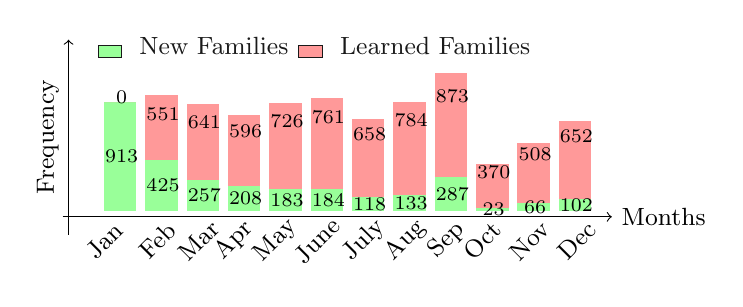
\begin{tikzpicture}[scale=1.5]

    \tikzstyle{every node}=[font=\small]
    % Scaling factor for the heights
    \def\scalefactor{0.001}
    
    % Define data for New and Learned Families
    \def\NewFamilies{{913, 425, 257, 208, 183, 184, 118, 133, 287, 23, 66, 102}}
    \def\LearnedFamilies{{0, 551, 641, 596, 726, 761, 658, 784, 873, 370, 508, 652}}

    % Define months
    \def\Months{{"Jan","Feb","Mar","Apr","May","Jun","Jul","Aug","Sep","Oct","Nov","Dec"}}
    
    % Loop through each month
    \foreach \x [count=\xi] in {0,...,11}{
        % Accessing the \x-th element of each list
        \pgfmathsetmacro\NewFamily{\NewFamilies[\x]}
        \pgfmathsetmacro\LearnedFamily{\LearnedFamilies[\x]}
        
        % Calculate bottom and top of the Learned Families bar
        \pgfmathsetmacro\NewHeight{\NewFamily*\scalefactor}
        \pgfmathsetmacro\LearnedHeight{(\NewFamily + \LearnedFamily)*\scalefactor}
        
        % Position for each month's data
        \pgfmathsetmacro\position{\xi*0.35}
        
        % Draw New Families (bottom bar)
        \fill[green!40] (\position,0) rectangle (\position+0.275,\NewHeight);
        % Draw Learned Families (stacked on top of New Families)
        \fill[red!40] (\position,\NewHeight) rectangle (\position+0.275,\LearnedHeight);
        
        % Add value labels for New and Learned Families
        \node at (\position+0.15,\NewHeight/2) {\scriptsize\NewFamily};
        % Display LearnedFamily value only if it's greater than 0
        \ifnum\LearnedFamily = 0
            \node at (\position+0.15,\LearnedHeight*1.05) {\scriptsize\LearnedFamily};
        \fi
         \ifnum\LearnedFamily > 0
            \node at (\position+0.15,\LearnedHeight/1.2) {\scriptsize\LearnedFamily};
        \fi
    }
     % Add month label below the x-axis
    %\node[rotate=45] at (\position+0.15,-0.2) {\tiny\Months[\x]};


    \node[rotate=45] at (0.35,-0.25) {Jan};
    \node[rotate=45] at (0.8,-0.25) {Feb};
    \node[rotate=45] at (1.15,-0.25) {Mar};
    \node[rotate=45] at (1.45,-0.25) {Apr};
    \node[rotate=45] at (1.80,-0.25) {May};
    \node[rotate=45] at (2.15,-0.25) {June};
    \node[rotate=45] at (2.55,-0.25) {July};
    \node[rotate=45] at (2.90,-0.25) {Aug};
    \node[rotate=45] at (3.25,-0.25) {Sep};
    \node[rotate=45] at (3.55,-0.25) {Oct};
    \node[rotate=45] at (3.95,-0.25) {Nov};
    \node[rotate=45] at (4.35,-0.25) {Dec};


    % Draw the axes
    \draw[->] (0.0,-0.05) -- (4.65,-0.05) node[right] {Months};
    \draw[->] (0.05,-0.2) -- (0.05,1.45) node[rotate=90, midway, above] {Frequency};
    

    % Add legends (moved to top right)
    \draw [black!90, fill=green!40] (.3,1.3) rectangle (0.5,1.4) node[right, xshift=0.1cm] {\small New Families};
    \draw [black!90, fill=red!40] (2.0,1.3) rectangle (2.20,1.4) node[right, xshift=0.1cm] {\small Learned Families};
    
\end{tikzpicture}


\vskip -0.1cm
\caption{New and already learned families in each task.}
\label{fig:ember_frequency_families}
\end{minipage}%
\vspace{-0.3cm}
\end{figure}




In this section, we provide an analysis of the EMBER dataset, which sheds light on the distribution across various families and tasks, aiding in selecting representative samples for replay. We identified 2,899 unique malware families within a subset of EMBER, and an additional 11,433 samples lacking clear family labels were assigned the label {\em Other}.

We investigate the prevalence of malware families over time, distinguishing between recurring and newly identified families each month in Figure~\ref{fig:ember_frequency_families}. Unlike many datasets used in CL research, we see significant churn in the representation of families over time. Of the 913 families seen in January, for example, only 551 are seen in February, while 425 new families emerge. This churn indicates a potential issue in training data continuity, which may aggravate catastrophic forgetting and underscores the need for different CL strategies in the malware domain. Table~\ref{ember_task_family_stat} shows the number of goodware and malware samples in each month, as well as the number of families. Generally, each family has its own distinct distribution pattern, and together these patterns make up the total distribution of malware for a particular month. 

Worse, many malware samples do not have family labels at all (see Figure~\ref{fig:ember_noavclass}). Correctly labeling samples is a challenging endeavor and often takes time and expert knowledge~\cite{kantchelian2015better}, so this lack of labels matches real-world conditions. Family labels for malware are based on the {\em av-class} labels provided by the av-test engine~\cite{av-test}. Analysis of the \emph{Other}-labeled samples do not align with the labeled families, which shows that many of them indeed come from unknown families. 


\begin{table}
\scriptsize
\centering
\caption{Number of samples and families per task in EMBER}
\begin{tabular}{l|c|c|c} 
% \hline \hline
\textbf{Task} & \textbf{\#of Goodware} & \textbf{\#of Malware} & \textbf{\#of Families}\\ 
\hline
%\rule{0pt}{2ex}

January     &   29423   &   32491    &  913       \\
February    &   22915   &   31222    &  976      \\
March       &   21373   &   20152    &  898      \\
April       &   25190   &   26892    &  804      \\
May         &   23719   &   22193    &  909      \\
June        &   23285   &   25116    &  945      \\
July        &   24799   &   26622    &  776      \\
August      &   23634   &   21791    &  917      \\
September   &   26707   &   37062    &  1160      \\
October     &   29955   &   56459    &  393      \\
November    &   50000   &   50000    &  574      \\
December    &   50000   &   50000    &  754      \\

\bottomrule

%\rule{0pt}{3ex}
\end{tabular}
\label{ember_task_family_stat}
\vskip -0.4cm   
\end{table}



\begin{figure}[t]
\begin{minipage}[c]{\linewidth}
\centering
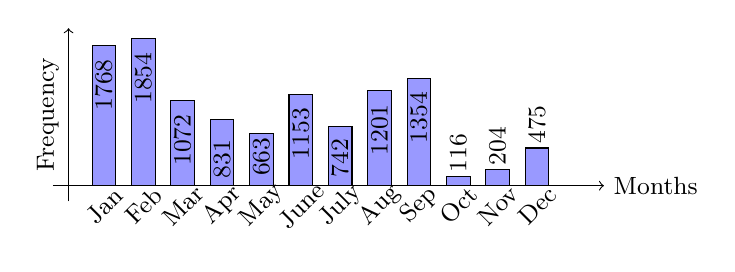
\begin{tikzpicture}[scale=1.]
    % Define the style for the bars and nodes
    \tikzstyle{every node}=[font=\small]
    %\tikzset{bar width/.initial=10pt}
    
    % Scaling factor for the heights
    \newcommand{\scalefactor}{0.001}
    
    % Drawing the bars for each month with reduced space
    \draw[fill=blue!40] (0,0) rectangle (0.3,1768*\scalefactor); % Jan
    \draw[fill=blue!40] (0.5,0) rectangle (0.8,1854*\scalefactor); % Feb
    \draw[fill=blue!40] (1,0) rectangle (1.3,1072*\scalefactor); % Mar
    \draw[fill=blue!40] (1.5,0) rectangle (1.8,831*\scalefactor); % Apr
    \draw[fill=blue!40] (2,0) rectangle (2.3,663*\scalefactor); % May
    \draw[fill=blue!40] (2.5,0) rectangle (2.8,1153*\scalefactor); % Jun
    \draw[fill=blue!40] (3,0) rectangle (3.3,742*\scalefactor); % Jul
    \draw[fill=blue!40] (3.5,0) rectangle (3.8,1201*\scalefactor); % Aug
    \draw[fill=blue!40] (4,0) rectangle (4.3,1354*\scalefactor); % Sep
    \draw[fill=blue!40] (4.5,0) rectangle (4.8,116*\scalefactor); % Oct
    \draw[fill=blue!40] (5,0) rectangle (5.3,204*\scalefactor); % Nov
    \draw[fill=blue!40] (5.5,0) rectangle (5.8,475*\scalefactor); % Dec
    
    % Add slanted labels below each bar for months
    \node[rotate=45] at (0.15,-0.25) {Jan};
    \node[rotate=45] at (0.65,-0.25) {Feb};
    \node[rotate=45] at (1.15,-0.25) {Mar};
    \node[rotate=45] at (1.65,-0.25) {Apr};
    \node[rotate=45] at (2.15,-0.25) {May};
    \node[rotate=45] at (2.65,-0.25) {June};
    \node[rotate=45] at (3.15,-0.25) {July};
    \node[rotate=45] at (3.65,-0.25) {Aug};
    \node[rotate=45] at (4.15,-0.25) {Sep};
    \node[rotate=45] at (4.65,-0.25) {Oct};
    \node[rotate=45] at (5.15,-0.25) {Nov};
    \node[rotate=45] at (5.65,-0.25) {Dec};
    
    % Add vertical frequency labels above each bar
    \node[rotate=90] at (0.15,1768*\scalefactor-0.5) {1768};
    \node[rotate=90] at (0.65,1854*\scalefactor-0.5) {1854};
    \node[rotate=90] at (1.15,1072*\scalefactor-0.5) {1072};
    \node[rotate=90] at (1.65,831*\scalefactor-0.5) {831};
    \node[rotate=90] at (2.15,663*\scalefactor-0.3) {663};
    \node[rotate=90] at (2.65,1153*\scalefactor-0.5) {1153};
    \node[rotate=90] at (3.15,742*\scalefactor-0.4) {742};
    \node[rotate=90] at (3.65,1201*\scalefactor-0.5) {1201};
    \node[rotate=90] at (4.15,1354*\scalefactor-0.5) {1354};
    \node[rotate=90] at (4.65,116*\scalefactor+0.3) {116};
    \node[rotate=90] at (5.15,204*\scalefactor+0.3) {204};
    \node[rotate=90] at (5.65,475*\scalefactor+0.3) {475};
    
    % Draw the axes
    \draw[->] (-0.5,0) -- (6.5,0) node[right] {Months};
    
    % Draw the y-axis with label alongside
    \draw[->] (-0.3,-0.2) -- (-0.3,2) node[rotate=90, midway, above] {Frequency};
    
\end{tikzpicture}



\vskip -0.25cm
\caption{EMBER Malware samples without AV-Class labels.}
\label{fig:ember_noavclass}
\end{minipage}%
\vskip -0.4cm
\end{figure}


% Furthermore, we also carried out an analysis to examine how consistently the top malware families appeared across different tasks. This helps us track the trends among the most common malware families in the EMBER dataset. For each task, we identified the 10 most common malware families, determined by the frequency of samples from each family. Our analysis show that the top 10 families changes over time, as the most prevalent families at the start did not stay prevalent in later tasks. For example, the \texttt{emotet} malware family was the most consistent, appearing in 11 out of 12 tasks. The next most consistent families were \texttt{fareit} and \texttt{zusy}, appearing in eight and seven of the tasks, respectively. This shows considerable concept drift in malware data, making it necessary to regularly update classifiers.

Furthermore, our analysis shows that the prominent malware families change with the evolution of tasks. We identified the 10 most common malware families based on the frequency of samples from each family and found that the top 10 families vary across tasks. The most prevalent families at the beginning of the experiment (i.e., January) do not remain prevalent in later tasks (i.e., from February on). For example, the \texttt{emotet} malware family was the most consistent, appearing in 11 out of 12 tasks. The next most consistent families were \texttt{fareit} and \texttt{zusy}, appearing in eight and seven tasks, respectively. This indicates considerable concept drift in malware data, highlighting the need to regularly update classifiers.

In addition, many malware families display complex distributional patterns in feature space, making for additional diversity within classes. Figure~\ref{fig:ember_jan_mal}, for example, shows a t-SNE projection of the EMBER features for all malware samples from January 2018. Each class (represented by color) is not clustered into a single well-defined region. Rather, the larger classes are split up into subsets that spread out in feature space. To accurately represent the malware distribution, it is thus important to select samples not only from each class, but also from multiple areas within each class.

Despite some degree of overlap among different families, it is possible to discern distinct clusters indicative of the diversity across and even within malware families. It is vital to capture samples from each of these smaller clusters, including those belonging to minority families, to accurately represent the malware landscape for a specific task month. 
To further complicate the situation, it is often not possible to provide definitive family labels for a sample due to the inherent subjectivity involved in malware analysis, which results in a large, diverse set of additional unlabeled samples which must be considered~\cite{kantchelian2015better}. These attributes of the malware landscape make it difficult to characterize classes as contiguous regions of the feature space with relatively simple class boundaries. Rather, each class might only be understood as a collection of smaller pockets of the feature space that might be closer to pockets from other classes than the same class. This may explain why prior CL techniques designed for computer vision datasets are less effective when applied to the malware domain~\cite{continual-learning-malware}. 



% These family-specific distributions are, in essence, sub-distributions of a broader global distribution, which underscores the significant diversity in real-world malware. 
%To further complicate the situation, many malware samples do not have family labels and correctly labeling samples often takes time and expert knowledge~\cite{kantchelian2015better}, so the lack of labels matches real-world conditions. %(see Figure~\ref{fig:ember_noavclass}). Family labels for malware are 
%based on the {\em av-class} labels 
%provided by the av-test engine~\cite{av-test}. %The \emph{other}-labeled samples indeed do not seem from our analysis to align with other families, meaning that many of them come from unknown families. 



% Table~\ref{ember_task_family_stat} provides a snapshot of the count of goodware and malware samples for each month, along with the unique malware families encountered in the corresponding month.


%\begin{table}[!t]
\small
% \def\arraystretch{1.35}
\centering
\caption{Top 10 most frequent malware families among 12 task months of EMBER.}
\vspace{-0.25cm}
\begin{tabular}{l|c||l|c}
% \toprule
\textbf{Family} & \textbf{Frequency} & \textbf{Family} & \textbf{Frequency} \\ \hline
Emotet & 11 & Upatre & 5 \\ 
Fareit & 8 & Installmonster & 4 \\
High & 8 &  zbot & 4\\ 
Zusy & 7 & Gandcrab & 3 \\ 
Adposhel & 4 & dealply & 3\\ 
\bottomrule
\end{tabular}
\label{tab:top10_families}
\vspace{-0.3cm}
\end{table}



\begin{figure}[!t]
\centering
\vskip -0.3cm
\includegraphics[scale=0.20,trim={0.5cm 0.8cm 0.5cm 0.5cm},clip]{figures/tsne_db_scan_mal.png}
\vskip -0.3cm
\caption{t-SNE projection of EMBER malware from Jan. 2018.}
\label{fig:ember_jan_mal}
\vskip -0.4cm
\end{figure}


%, which is a challenging issue in its own right~\cite{cade,transcendingtranscend} that continual learning methods should address. 

In light of these analysis, we propose that selecting samples based on families and variations within those families could more effectively capture the diversity within the replay data distribution, potentially mitigating catastrophic forgetting. 







\section{Diversity-Aware Replay}
\label{divreplay}

Here, we introduce the our proposed continual learning (CL) framework for malware classification with two diversity-aware replay variants: MADAR and MADAR$^\theta$. MADAR operates on the basis of the raw-feature space and MADAR$^\theta$ operates on the basis of the model's weights-space of raw-features. 



\subsection{MADAR}
\label{subsec:ifs}

% GRS is implicitly designed on the assumption that important information for training is distributed evenly across the dataset. We instead aim to sample intelligently to capture key information while avoiding unnecessary redundancy. Building on the dataset analysis in Section~\ref{sec:exploratoryAnalysis}, we postulate that stratified sampling, where replay samples are chosen based on their representation in malware families, might better preserve the model's stability than random sampling. Moreover, we also seek to capture the diversity \emph{within} the malware family data distribution. This entails incorporating both \emph{representative} samples that are close to the centroid and \emph{discriminative} samples that lie further from the centroid into the replay sample pool. To this end, we conjecture that a technique for identifying outliers within a distribution could effectively pinpoint the most discriminative samples, while a random subset of non-outliers would address a variety of representative samples without excess redundancy.

% GRS assumes even distribution of important information across the dataset, while we propose intelligent stratified sampling.

Building on the exploratory analysis in Section~\ref{sec:exploratoryAnalysis}, we postulate that stratified sampling, where replay samples are chosen based on their representation in malware families, may better preserve the model's stability versus random sampling as used in GRS. Moreover, we also seek to capture the diversity \emph{within} each family's data distribution. 
%As such, our proposed techniques are designed to provide replay samples from each individual malware family distribution by choosing 
We do this by selecting a balance between \emph{representative samples} that are close to each other and \emph{anomalous samples} that are separated. 
%In particular, the samples that may form a cluster can be termed as the representative samples of the cluster and the samples that do not necessarily form a cluster or the samples which are farther away from the formed cluster can be termed as the outliers in this context. It is important for a malware classifier to not forget these outliers because these outliers are still crucial as they maybe very few in number and may have less overlap in the code compared to other samples of a particular family. 
While any single anomalous sample is not as important to learn and remember as a single representative sample, a collection of anomalous samples helps to track the diversity within a class.
%And forgetting these samples may increase {false negatives}. As such, our techniques preserve representation of the similar samples and outlier samples to retain the inner diversity of a family.
% We capture diversity within malware families by including representative samples near the centroid and discriminative samples farther away. Outlier identification helps pinpoint discriminative samples, while a random subset of non-outliers provides representative diversity without redundancy.


% {\em Isolation Forests (IF)}\cite{if} are an efficient approach to finding outliers in high-dimensional data like our malware dataset. IF employs decision trees to randomly select a feature and split value, producing shorter paths for anomalous data points and distinguishing them from the rest of the data. This approach stems from the intuition that anomalous data points are few, distinct, and easy to isolate. In IF, data samples are partitioned by randomly selecting a feature $f$ and recursively splitting the samples until they are completely isolated from one another. The resulting path lengths are used to rank each sample based on their degree of anomaly, yielding anomaly scores that can be used to pinpoint outliers. An important parameter of IF is the contamination rate $C_{r}$, $0 \leq C_{r} \leq 0.5$ -- the anticipated fraction of outlier samples in the distribution. After experimenting with $C_{r} \in \{0.1, .., 0.5\}$, we observe that $C_{r} = 0.1$ was the best, and we thus use $C_{r} = 0.1$ in all of our experiments.

{\em Isolation Forest (IF)}~\cite{if} is a technique for identifying outliers in high-dimensional data. IF uses decision trees to isolate anomalous data points based on the intuition that outliers are distinct and easy to separate from the rest of the data. An important parameter in IF is the contamination rate $C_{r}$, which represents the expected fraction of outliers in the data. We found that $C_{r} = 0.1$ works best and used it in all our experiments. The algorithm for \system\ in the Domain-IL setting is provided in Algorithm~\ref{alg:IFS}. The algorithm for \system\ in the Class-IL and Task-IL settings is provided in Algorithm~\ref{alg:IFS_Class_Task_IL}. 


\begin{algorithm}[!t]
\small
% functions
\SetKwFunction{cumprod}{cumprod}
\SetKwFunction{length}{length}
\SetKwFunction{zeros}{zeros}
\SetKwFunction{ceil}{ceil}
% input/ouput names
\SetKwInOut{Input}{Input}
\SetKwInOut{Output}{Output}
% caption
\caption{~\system~in Domain-IL. 
\label{alg:IFS}}
\Input{
    $c$ -- Current Task number, $X_{c}, Y_{c}$ -- Samples and labels of $c$, 
    $\mathcal{P}$ -- Data pool, 
    $\beta$ -- Memory budget,  $\gamma$ -- Split of $\beta$ for malware and goodware, 
    $\Omega$ -- Split of anomalous/similar samples, 
    $\xi$ -- Ratio budgeting, $\Psi$ -- Uniform budgeting
}


% \Input{%
% 		\xvbox{20mm}{$c$} -- Current task number \\
%         \xvbox{20mm}{$X_{c}, Y_{c}$} -- Samples and labels of $c$\\
% 		\xvbox{20mm}{$\mathcal{P}$} -- Data pool \\
% 		\xvbox{20mm}{$\beta$} -- Memory budget \\
%             \xvbox{3mm}{$\gamma$} -- Split of $\beta$ for malware and goodware \\
%             \xvbox{3mm}{$\Omega$} -- Split of anomalous and similar samples \\
%             \xvbox{3mm}{$\xi$} -- Ratio budgeting \\
%             \xvbox{3mm}{$\Psi$} -- Uniform budgeting \\
    
  \BlankLine 

    \xvbox{14mm}{\texttt{\bf init~~} $\mathcal{P}$;}
    %{\tcp{Global data pool}}
    \xvbox{1mm}{\texttt{\bf init~~} $\mathcal{D} \leftarrow \{M_{f}: M_{c}\}$;}
    %{\tcp{Global dictionary of malware family $M_{f}$ and sample counts $M_{c}$ of $M_{f}$}}
    
    %\BlankLine
    \If{$c = 0$}{
        \xvbox{20mm}{$\mathcal{P} \leftarrow X_{c}, Y_{c}$;}
        
        \xvbox{20mm}{$X_{good}, X_{mal} \leftarrow  \mathcal{P}$;} 
        
        \xvbox{20mm}{$\nabla \mathcal{D} \leftarrow X_{mal}$}
        %{\tcp{Update global dictionary}}
        
        \xvbox{20mm}{$X_{train},~Y_{train} \leftarrow X_{c}, Y_{c}$}
        }
        
    %\BlankLine
    
    \Else{
        \xvbox{40mm}{$X_{good}, X_{mal} \leftarrow  \mathcal{P}$;} 
        % {\tcp*{Separate out goodware and malware samples from global family data pool}}
        
        \xvbox{22mm}{$\beta_M, \beta_G \leftarrow \beta~.~\gamma$;} %{\tcp{Malware and Goodware budgets}}

        \xvbox{26mm}{$\beta_A$, $\beta_S \leftarrow \beta_M~.~\Omega$;} %{\tcp{Budgets of anomalous and similar samples}}    
        
        %\BlankLine
        % \If{$\Psi$}{
        %             \xvbox{20mm}{$\mathcal{NF} \leftarrow \mathcal{D}$;}%{\tcp{\#of malware families in $\mathcal{D}$}}
                    
        %             \xvbox{37mm}{$\mathcal{B_{F}} \leftarrow \beta_M / \mathcal{NF}$;}
        %             %{\tcp{Family budget}}
        %             }

        \If{$\Psi$}{ % Uniform budgeting
            \xvbox{20mm}{$\mathcal{NF} \leftarrow |\mathcal{D}|$;} %{\tcp{\# of malware families in $\mathcal{D}$}}
            \xvbox{37mm}{$\mathcal{B_{F}} \leftarrow \beta_M / \mathcal{NF}$;} %{\tcp{Family budget}}
        }
        %\BlankLine

        
        
        \xvbox{28mm}{$R_{mal} \leftarrow [~]$;} %{\tcp{Malware replay samples}}
        \BlankLine
        \For{$X_{f} \subseteq X_{mal}$ %{~~~~~~~~\tcp{Each family \emph{\texttt{f}}}}
        }{
                \xvbox{20mm}{$\mathcal{F_{MC}} \leftarrow X_{f}$;}
                %{\tcp{\$of malware in $X_{f}$}}
                
                %\BlankLine
                \If{$\xi$}{
                    \xvbox{20mm}{$\mathcal{MC} \leftarrow |\mathcal{D}|$;}%{\tcp{Total \# of malware in $\mathcal{D}$}}
                    \xvbox{37mm}{$\mathcal{B_{F}} \leftarrow (\mathcal{F_{MC}} / \mathcal{MC}) * \beta_M$;}%{\tcp{Family budget}}
                }
                
                \If{$\mathcal{F_{MC}} <= \mathcal{B_{F}} $}{
                    \xvbox{20mm}{$R_{mal}.\texttt{append}(X_{f})$;}
                }

                \Else {
                    $({A}_f, {S}_f) \leftarrow \texttt{IF}(X_{f}, \beta_A, \beta_S);$ 
                    {%\tcp{Anomalous and Similar samples selected w/ IF}
                    }
                    
                    $R_{mal}.\texttt{append}({A}_f, {S}_f)$
                }
        }
        
        \xvbox{80mm}{$R_{good}  \leftarrow \texttt{sample}(X_{good}, \texttt{len}(R_{mal}))$;} 
        %{%\tcp{Randomly select as much goodware as malware}}
        %\BlankLine

        \xvbox{40mm}{$X_{replay}  \leftarrow (R_{good}, R_{mal})$;}
        
        \xvbox{40mm}{$Y_{replay}  \leftarrow ([0] * \texttt{len}(R_{good}), [1]*\texttt{len}(R_{mal}))$;}

        %\BlankLine
        
        \xvbox{40mm}{$X_{train}  \leftarrow \texttt{concat}((X_{c}, X_{replay}))$;}

        \xvbox{20mm}{$Y_{train}  \leftarrow (\texttt{concat}((Y_{c}, Y_{replay}))$;}

        %\BlankLine
        $\mathcal{P}.\texttt{append}(X_{c}, Y_{c})$; 
    $\nabla \mathcal{D} \leftarrow X_{mal}$;
        % \xvbox{28mm}{$\mathcal{P}.$ \texttt{append}$(X_{c}, Y_{c})$;}
        % {%\tcp{Update $\mathcal{P}$ with samples of current task}
        % }

        % \xvbox{28mm}{$\nabla \mathcal{D} \leftarrow X_{mal}$}{
        % %\tcp{Update global dictionary}
        % }
        
    }
    \texttt{\bf return} $(X_{train},~Y_{train})$
% \vspace{-0.2cm}
\end{algorithm}





% In IFS, presented in Algorithm~\ref{alg:IFS}, goodware and malware samples are treated separately, and malware samples are further selected based on families. We present IFS using Domain-IL for simplicity, and Class-IL follows the similar procedure. IFS initializes a global data pool $\mathcal{P}$ to preserve all the goodware samples and malware samples based on their family; and a dictionary $\mathcal{D}$ to preserve the name of family and the associated frequencies of malware samples till the current task.

% For any subsequent task, IFS separates goodware $X_{good}$ and malware $X_{mal}$ from $\mathcal{P}$. Afterwards, it allocates malware $\beta_M$ and goodware $\beta_G$ budgets from the memory budget $\beta$ based on a given split ratio of $\gamma$. If the dataset is relatively balanced in terms of goodware and malware which it is for EMBER, we can simply use $\gamma \in \{50:50\}$, however, if the dataset is not balanced which it is for AZ datasets, we can use a tuned $\gamma$. For AZ dataset, we use $\gamma \in \{90:10\}$. 

% In IFS, detailed in Algorithm~\ref{alg:IFS}, goodware and malware are processed separately, with malware further categorized by family.

\subsubsection*{\bf Procedure}
We now describe \system using the framework of Domain-IL; the process is similar for Class-IL and Task-IL. 
%\system processes goodware and malware separately, further categorizing malware by family. 
The procedure begins by initializing a global data pool $\mathcal{P}$, containing both goodware and malware samples, and a dictionary $\mathcal{D}$ that tracks malware families and their frequencies in the data up to the current task.

For each new task $c$, \system divides the data into goodware ($X_{good}$) and malware ($X_{mal}$) subsets from $\mathcal{P}$, allocating memory budgets $\beta_M$ for malware and $\beta_G$ for goodware from the total memory budget $\beta$, based on a split ratio $\gamma$:
\begin{equation}
    \beta_G = \gamma \cdot \beta, \quad  \beta_M = (1 - \gamma) \cdot \beta. %\nonumber
\end{equation}
For balanced datasets like EMBER, $\gamma = 0.5$ ensures an equal split between malware and goodware. For an imbalanced dataset, it is better to tune $\gamma$. Our Android malware (AZ) datasets, for example, have a 9:1 ratio of goodware to malware, so we use $\gamma=0.9$.

Before training for a new task, \system incrementally trains the classifier using a combination of new samples from the current task and replay samples from previous tasks. The replay samples include both goodware ($R_{good} \subset X_{good}$) and malware ($R_{mal} \subset X_{mal}$), with $R_{mal}$ sampled from specific malware families rather than randomly from all of $X_{mal}$.

For each family $f$, we set its \emph{family budget} $\mathcal{B}_f$---
the number of samples to select from $f$---using two sub-sampling variants: \emph{Ratio budgeting} and \emph{Uniform budgeting}. 


\begin{smitemize}
    \item \textbf{Ratio Budgeting:} Select the number of samples from a family $f$ proportional to that family's representation in the dataset. The family budget $\mathcal{B}_f$ is
    $\mathcal{B}_f = \frac{|X_{f}|}{|X_{mal}|} \cdot \beta_M$,
%    \begin{equation}
 %       \mathcal{B}_f = \frac{|X_{f}|}{|X_{mal}|} \cdot \beta_M
 %   \end{equation}
    %
    where $|X_{f}|$ is the number of samples in family $f$, and $|X_{mal}|$ is the total number of malware samples. This strategy may be more suitable in binary classification, as it provides proportional representation of the malware families for training on the malicious class.
    
    \item \textbf{Uniform Budgeting:} In this method, the memory budget $\beta_M$ is uniformly distributed across all malware families:
    %\begin{equation}
        $\mathcal{B}_f = \frac{\beta_M}{|\mathcal{F}|}$,
    %\end{equation}
    where $|\mathcal{F}|$ is the total number of malware families. 
    Compared with Ratio budgeting, Uniform budgeting may work well for multi-class classification to determine which family a sample belongs to, as it ensures better class balance.
\end{smitemize}

Within each family $f$, we further split the family budget $\mathcal{B}_f$ into two parts: representative samples $S_f$ and anomalous samples $A_f$, using IF, controlled by a split parameter $\alpha$:
\begin{equation}
    |S_f| = \alpha \cdot \mathcal{B}_f, \quad |A_f| = (1 - \alpha) \cdot \mathcal{B}_f %\nonumber 
\end{equation}
%Our experiments reveal that an even split, $\alpha = 0.5$, of representative and anomalous samples provides the optimal performance. 
%
We found empirically that a balanced split ($\alpha = 0.5$) between representative and anomalous samples provides optimal performance. In this setup, the model learns equally the core class characteristics from representative samples %($|S_f| = \alpha \cdot \mathcal{B}_f$) 
and less common variations from anomalous samples. 
%($|A_f| = (1 - \alpha) \cdot \mathcal{B}_f$), 
%allowing it to generalize well and handle edge cases equally well.
%without overemphasizing one type at the expense of the other. 
%We see no reason to expect that this setting would favor a highly imbalanced split in either direction.

The malware replay set $R_{mal}$ is then constructed by combining the representative and anomalous samples from all malware families: 
\begin{equation}
    R_{mal} = \bigcup_{f \in F} \{ S_f \cup A_f \}. %\nonumber 
\end{equation}
The total replay set consists of both goodware and malware replay samples, which are then concatenated with the new task samples
%The number of goodware samples in the replay set is chosen such that \(|R_{good}| = \beta_G \). 
%The replay samples and the new task samples are concatenated 
to form the training set for the current task $c$.
%$R = R_{good} \cup $
%\begin{equation}
%    X_{train} = X_c \cup X_{replay}, \quad Y_{train} = Y_c \cup Y_{replay}
%\end{equation}
After training, the data pool $\mathcal{P}$ is updated with the new task samples, \(\mathcal{P} \leftarrow \mathcal{P} \cup \{X_c, Y_c\}\), and the malware family dictionary $\mathcal{D}$ is updated to reflect the new frequencies of malware families in $X_{mal}$: \(\mathcal{D} \leftarrow \mathcal{D} + freq(X_{mal})\).



\begin{algorithm}[!t]
\small
\caption{\system~in Class-IL and Task-IL \label{alg:IFS_Class_Task_IL}}
\SetKwInOut{Input}{Input}
\SetKwInOut{Output}{Output}

\Input{
    $c$ -- Task number, $X_{c}, Y_{c}$ -- Malware samples and their family labels, 
    $\mathcal{P}$ -- Malware data pool, 
    $\beta$ -- Memory budget, 
    $\Omega$ -- Split of anomalous/similar samples, 
    $\xi$ -- Ratio budgeting, $\Psi$ -- Uniform budgeting
}

\xvbox{14mm}{\texttt{\bf init~~} $\mathcal{P}$;}
\xvbox{1mm}{\texttt{\bf init~~} $\mathcal{D} \leftarrow \{M_{f}: M_{c}\}$;}

\If{$c = 0$}{
    $\mathcal{P} \leftarrow X_{c}, Y_{c}$; 
    $X_{mal} \leftarrow \mathcal{P}$; 
    $\nabla \mathcal{D} \leftarrow X_{mal}$; 
    $X_{train}, Y_{train} \leftarrow X_{c}, Y_{c}$;
}

\Else{
    $X_{mal} \leftarrow \mathcal{P}$; 
    $\beta_A, \beta_S \leftarrow \beta \cdot \Omega$; 
    
    \If{$\Psi$}{
        $\mathcal{NF} \leftarrow \mathcal{D}$; 
        $\mathcal{B_F} \leftarrow \beta / \mathcal{NF}$;
    }
    
    $R_{mal} \leftarrow [~]$; 
    \For{$X_{f} \subseteq X_{mal}$}{
        $\mathcal{F_{MC}} \leftarrow X_{f}$; 
        \If{$\xi$}{
            $\mathcal{MC} \leftarrow \mathcal{D}$; 
            $\mathcal{B_F} \leftarrow (\mathcal{F_{MC}} / \mathcal{MC}) \cdot \beta$;
        }
        \If{$\mathcal{F_{MC}} \leq \mathcal{B_F}$}{
            $R_{mal}.\texttt{append}(X_{f})$;
        } \Else{
            $({A}_f, {S}_f) \leftarrow \texttt{IF}(X_{f}, \beta_A, \beta_S)$; 
            $R_{mal}.\texttt{append}({A}_f, {S}_f)$;
        }
    }
    
    $X_{replay} \leftarrow R_{mal}$; 
    $Y_{replay} \leftarrow ([1] \times \texttt{len}(R_{mal}))$; 

    $X_{train} \leftarrow \texttt{concat}(X_{c}, X_{replay})$; 
    $Y_{train} \leftarrow \texttt{concat}(Y_{c}, Y_{replay})$;
    
    $\mathcal{P}.\texttt{append}(X_{c}, Y_{c})$; 
    $\nabla \mathcal{D} \leftarrow X_{mal}$;
}
\textbf{return} $(X_{train}, Y_{train})$
\end{algorithm}



%%%%%%%%% AsiaCCS V1 %%%%%%%%

% \begin{algorithm}
% \caption{\system~for Class-IL and Task-IL}
% \label{alg:IFS_Class_Task_IL}
% \begin{algorithmic}[1]
% \REQUIRE $c$ -- Task number, $X_{c}, Y_{c}$ -- Malware samples and family labels, 
% $\mathcal{P}$ -- Malware data pool, $\beta$ -- Memory budget, $\Omega$ -- Split of anomalous/similar samples, 
% $\xi$ -- Ratio budgeting, $\Psi$ -- Uniform budgeting
% \ENSURE $(X_{train}, Y_{train})$

% \STATE \textbf{Initialize:} $\mathcal{P}$, $\mathcal{D} \leftarrow \{M_{f}: M_{c}\}$
% \IF{$c = 0$}
%     \STATE $\mathcal{P} \leftarrow X_{c}, Y_{c}$
%     \STATE $X_{mal} \leftarrow \mathcal{P}$
%     \STATE $\nabla \mathcal{D} \leftarrow X_{mal}$
%     \STATE $X_{train}, Y_{train} \leftarrow X_{c}, Y_{c}$
% \ELSE
%     \STATE $X_{mal} \leftarrow \mathcal{P}$
%     \STATE $\beta_A, \beta_S \leftarrow \beta \cdot \Omega$
%     \IF{$\Psi$}
%         \STATE $\mathcal{NF} \leftarrow \mathcal{D}$
%         \STATE $\mathcal{B_F} \leftarrow \beta / \mathcal{NF}$
%     \ENDIF
%     \STATE $R_{mal} \leftarrow [~]$
%     \FOR{$X_{f} \subseteq X_{mal}$}
%         \STATE $\mathcal{F_{MC}} \leftarrow X_{f}$
%         \IF{$\xi$}
%             \STATE $\mathcal{MC} \leftarrow \mathcal{D}$
%             \STATE $\mathcal{B_F} \leftarrow (\mathcal{F_{MC}} / \mathcal{MC}) \cdot \beta$
%         \ENDIF
%         \IF{$\mathcal{F_{MC}} \leq \mathcal{B_F}$}
%             \STATE $R_{mal}.\texttt{append}(X_{f})$
%         \ELSE
%             \STATE $({A}_f, {S}_f) \leftarrow \texttt{IF}(X_{f}, \beta_A, \beta_S)$
%             \STATE $R_{mal}.\texttt{append}({A}_f, {S}_f)$
%         \ENDIF
%     \ENDFOR
%     \STATE $X_{replay} \leftarrow R_{mal}$
%     \STATE $Y_{replay} \leftarrow ([1] \times \texttt{len}(R_{mal}))$
%     \STATE $X_{train} \leftarrow \texttt{concat}(X_{c}, X_{replay})$
%     \STATE $Y_{train} \leftarrow \texttt{concat}(Y_{c}, Y_{replay})$
%     \STATE $\mathcal{P}.\texttt{append}(X_{c}, Y_{c})$
%     \STATE $\nabla \mathcal{D} \leftarrow X_{mal}$
% \ENDIF
% \STATE \textbf{return} $(X_{train}, Y_{train})$
% \end{algorithmic}
% \end{algorithm}


%%%%%%%%

% \begin{algorithm}[!t]
% \small
% \caption{\system~in Class-IL and Task-IL \label{alg:IFS_Class_Task_IL}}
% \SetKwInOut{Input}{Input}
% \SetKwInOut{Output}{Output}

% \Input{
%     $c$ -- Task number, $X_{c}, Y_{c}$ -- Malware samples and their family labels, 
%     $\mathcal{P}$ -- Malware data pool, 
%     $\beta$ -- Memory budget, 
%     $\Omega$ -- Split of anomalous/similar samples, 
%     $\xi$ -- Ratio budgeting, $\Psi$ -- Uniform budgeting
% }

% \xvbox{14mm}{\texttt{\bf init~~} $\mathcal{P}$;}
% \xvbox{1mm}{\texttt{\bf init~~} $\mathcal{D} \leftarrow \{M_{f}: M_{c}\}$;}

% \If{$c = 0$}{
%     $\mathcal{P} \leftarrow X_{c}, Y_{c}$; 
%     $X_{mal} \leftarrow \mathcal{P}$; 
%     $\nabla \mathcal{D} \leftarrow X_{mal}$; 
%     $X_{train}, Y_{train} \leftarrow X_{c}, Y_{c}$;
% }

% \Else{
%     $X_{mal} \leftarrow \mathcal{P}$; 
%     $\beta_A, \beta_S \leftarrow \beta \cdot \Omega$; 
    
%     \If{$\Psi$}{
%         $\mathcal{NF} \leftarrow \mathcal{D}$; 
%         $\mathcal{B_F} \leftarrow \beta / \mathcal{NF}$;
%     }
    
%     $R_{mal} \leftarrow [~]$; 
%     \For{$X_{f} \subseteq X_{mal}$}{
%         $\mathcal{F_{MC}} \leftarrow X_{f}$; 
%         \If{$\xi$}{
%             $\mathcal{MC} \leftarrow \mathcal{D}$; 
%             $\mathcal{B_F} \leftarrow (\mathcal{F_{MC}} / \mathcal{MC}) \cdot \beta$;
%         }
%         \If{$\mathcal{F_{MC}} \leq \mathcal{B_F}$}{
%             $R_{mal}.\texttt{append}(X_{f})$;
%         } \Else{
%             $({A}_f, {S}_f) \leftarrow \texttt{IF}(X_{f}, \beta_A, \beta_S)$; 
%             $R_{mal}.\texttt{append}({A}_f, {S}_f)$;
%         }
%     }
    
%     $X_{replay} \leftarrow R_{mal}$; 
%     $Y_{replay} \leftarrow ([1] \times \texttt{len}(R_{mal}))$; 

%     $X_{train} \leftarrow \texttt{concat}(X_{c}, X_{replay})$; 
%     $Y_{train} \leftarrow \texttt{concat}(Y_{c}, Y_{replay})$;
    
%     $\mathcal{P}.\texttt{append}(X_{c}, Y_{c})$; 
%     $\nabla \mathcal{D} \leftarrow X_{mal}$;
% }
% \textbf{return} $(X_{train}, Y_{train})$
% \end{algorithm}





\subsection{MADAR$^\theta$}
\label{subsec:aws}





While Isolation Forest (IF) outperforms other distance-based anomaly detection techniques on high-dimensional data, it struggles with correlated features~\cite{puggini2018enhanced}. Let \( \mathbf{X} \in \mathbb{R}^D \) represent the input data, where \( D \) is the feature dimension. For example, the EMBER dataset has \( D = 2381 \), while the AZ datasets have \( D = 1789 \) for AZ-Domain and \( D = 2439 \) for AZ-Class, respectively. Instead of applying dimensionality reduction techniques such as PCA, we propose leveraging a neural network \( \mathcal{M} \) to generate compact feature representations \( \mathbf{Z} \in \mathbb{R}^d \), where \( d \ll D \). This approach is particularly advantageous in continual learning contexts, as it complements ongoing model development and adapts to evolving tasks~\cite{hayes2020remind,ostapenko2022foundational}.

To address these, we introduce MADAR$^\theta$, a variant of MADAR that leverages learned representations from a trained model \( \mathcal{M} \) to identify both representative and diverse samples effectively. 
%The MADAR$^\theta$ algorithm is provided in Appendix~\ref{append:awsAlgo}. 
For an input sample \( \mathbf{x} \), the model \( \mathcal{M} \) computes activations \( \mathcal{W}(\mathbf{x}) \), representing its internal state. Specifically, for a set of inputs \( \mathbf{X}_f \) belonging to a family \( f \), MADAR$^\theta$ extracts activations:
\begin{equation}
\Theta^\mathcal{L}(\mathbf{X}_f) = \{ \mathcal{W}^\mathcal{L}(\mathbf{x}) : \mathbf{x} \in \mathbf{X}_f \}, \quad \text{where} \quad \Theta^\mathcal{L}(\mathbf{X}_f) \in \mathbb{R}^d,
\end{equation}
from a chosen layer \( \mathcal{L} \) of the model.

These activations are analyzed using the Isolation Forest (IF) algorithm to identify anomalous activations \( \mathcal{A}_w \subseteq \Theta^\mathcal{L}(\mathbf{X}_f) \). The corresponding anomalous samples in the original input space are denoted as:
\begin{equation}
A_f = \{ \mathbf{x} \in \mathbf{X}_f : \mathcal{W}^\mathcal{L}(\mathbf{x}) \in \mathcal{A}_w \}.
\end{equation}
Non-anomalous samples are similarly sampled to form the set \( S_f \), ensuring a balanced and representative replay set:
\begin{equation}
S_f = \{ \mathbf{x} \in \mathbf{X}_f : \mathcal{W}^\mathcal{L}(\mathbf{x}) \notin \mathcal{A}_w \}.
\end{equation}

The replay samples \( A_f \cup S_f \) are then used in subsequent training episodes to maintain knowledge retention and mitigate catastrophic forgetting.

\paragraphX{Selection of the Layer \( \mathcal{L} \).}
The choice of \( \mathcal{L} \) is critical in MADAR$^\theta$ to ensure that feature representations are captured without interference from the model's final classification stage. Empirical testing revealed that the penultimate layers, denoted as \texttt{act4} for the EMBER dataset and \texttt{act5} for the AZ datasets, provide optimal results such that $\mathcal{L}_{\text{EMBER}} = \texttt{act4}, \quad \mathcal{L}_{\text{AZ}} = \texttt{act5}.$

% \begin{equation}
% \mathcal{L}_{\text{EMBER}} = \texttt{act4}, \quad \mathcal{L}_{\text{AZ}} = \texttt{act5}.
% \end{equation}

\paragraphX{Adaptation of Batch Normalization.}
During the forward pass, batch normalization is omitted in MADAR$^\theta$ to preserve the diversity of the activation distributions. While batch normalization typically stabilizes learning and improves generalization, it can homogenize activations, reducing the diversity essential for identifying anomalies. This adaptation enhances the performance of MADAR$^\theta$, as confirmed by empirical results.


% \begin{equation}
% \Theta^\mathcal{L}(\mathbf{X}_f) = \text{ForwardPass}(\mathbf{X}_f, \text{BatchNorm=False}).
% \end{equation}




\paragraphX{Efficiency of MADAR$^\theta$.}
MADAR$^\theta$ is computationally efficient compared to MADAR applied directly to the input space. The hidden layers \texttt{act4} and \texttt{act5} have \( d = 128 \), significantly reducing the dimensionality from \( D \). As a result, MADAR$^\theta$ offers reduced computational complexity.

% \begin{equation}
% \text{Time Complexity of IF} \propto \mathcal{O}(d \log n),
% \end{equation}
% where \( n \) is the number of samples. This efficiency further underscores the practicality of MADAR$^\theta$ for continual learning scenarios.






% While IF works better than other distance-based anomaly detection techniques on high-dimensional data, it can struggle with correlated features~\cite{puggini2018enhanced}. The EMBER dataset has 2,381 features, and while the AZ datasets have 1,789 and 2,439 features for AZ-Domain and AZ-Class, respectively. Instead of applying dimensionality reduction, leveraging the neural network to generate a more compact feature representation could be a beneficial approach, especially in continual-learning contexts where it complements ongoing model development efforts~\cite{hayes2020remind,ostapenko2022foundational}. 

% As such, we introduce MADAR$^\theta$ which is based on anomalous weights, a variant of MADAR that leverages learned representations from a trained model, $\mathcal{M}$, to more effectively identify both representative and diverse samples. 
% %A schematic representation of AWS is depicted in Figure~\ref{fig:madar-aws}. 
% By inputting a sample $\mathcal{X}$ into $\mathcal{M}$, we obtain activations $\mathcal{W}$ reflecting the sample's internal state. For inputs $X_{f}$ from family $f$, MADAR$^\theta$ extracts activations $\Theta^{L}{X_{f}} \in \mathbb{R}^{D}$ from a chosen layer $\mathcal{L}$. These activations are then analyzed with the Isolation Forest (IF) algorithm to pinpoint anomalous activations, $\mathcal{A}_{w}$. MADAR$^\theta$ then maps these anomalies back to the original input space of $X_{f}$ to select the anomalous samples $A_f$. Non-anomalous samples are similarly sampled to form $S_f$. Aside from these steps, MADAR$^\theta$ proceeds similarly to MADAR. 

% In selecting the layer $\mathcal{L}$ for MADAR$^\theta$, we aim to capture feature representations while avoiding the model's final classification stage. Testing various layers revealed that the penultimate layers, \texttt{act4} for EMBER and \texttt{act5} for AZ, yield the best results. Thus, we utilized these layers for the remainder of our study. We also adapted the MADAR$^\theta$ algorithm by omitting batch normalization during the forward pass. Although batch normalization generally stabilizes learning and improves model generalization by normalizing input layers, in the MADAR$^\theta$ context, it can diminish the activation distribution diversity we seek to maintain. Our tests confirmed that excluding batch normalization enhances MADAR$^\theta$'s performance.

% Besides enhancing replay sample selection, MADAR$^\theta$ is also more efficient than IFS. The \texttt{act4} and \texttt{act5} hidden layers have just 128 dimensions each, considerably less than the original feature dimensions. The IF algorithm thus operates more quickly in this reduced dimension space.


% \input{5_1_experimental_details}
\section{Evaluation}

% \saidur{Working on it}




\begin{table*}[!t]
% \small
\centering
\caption{Summary of Results for EMBER Domain-IL Experiments.}
\vspace{-0.2cm}
\label{tab:ember_DIL}

\begin{tabular}{p{1.1cm}|l|c|c|c|c|c|c|c} 

% \toprule 

\multirow{2}{*}{\textbf{Group}} & \multirow{2}{*}{\textbf{Method}} & \multicolumn{7}{c}{\textbf{Budget}} \\ \cline{3-9}

&  & 1K & 10K & 50K & 100K & 200K & 300K & 400K \\ \midrule

\multirow{3}{*}{Baselines} 
& Joint  & \multicolumn{7}{c}{96.4$\pm$0.3} \\ 
& None   & \multicolumn{7}{c}{93.1$\pm$0.1} \\ 
& GRS    & 93.6$\pm$0.3 & 94.1$\pm$1.3 & 95.3$\pm$0.2 & 95.3$\pm$0.7 & 95.9$\pm$0.1 & 95.8$\pm$0.6 & 96.0$\pm$0.3 \\ 
\midrule

\multirow{4}{*}{\parbox{0.7cm}{Prior \\ Work}} 
& ER~\cite{er}     & 80.6$\pm$0.1 & 73.5$\pm$0.5 & 70.5$\pm$0.3 & 69.9$\pm$0.1 & 70.0$\pm$0.1 & 70.0$\pm$0.1 & 70.0$\pm$0.1 \\ 
& AGEM~\cite{agem}   & 80.5$\pm$0.1 & 73.6$\pm$0.2 & 70.4$\pm$0.3 & 70.0$\pm$0.1 & 70.0$\pm$0.2 & 70.0$\pm$0.1 & 70.0$\pm$0.1 \\ 
& GR~\cite{gr}     & \multicolumn{7}{c}{93.1$\pm$0.2} \\ 
& RtF~\cite{rtf}    & \multicolumn{7}{c}{93.2$\pm$0.2} \\ 
& BI-R~\cite{BIR}   & \multicolumn{7}{c}{93.4$\pm$0.1} \\ 
\midrule

\multirow{4}{*}{\system}      
& \system-R         & \textbf{93.7$\pm$0.1} & \textbf{94.7$\pm$0.1} & \textbf{95.4$\pm$0.1} & \textbf{95.3$\pm$0.6} & \textbf{96.0$\pm$0.1} & \textbf{96.1$\pm$0.1} & \textbf{96.1$\pm$0.1} \\ 
& \system-U         & \textbf{93.6$\pm$0.2} & 94.0$\pm$0.2 & 95.1$\pm$0.1 & \textbf{95.3$\pm$0.1} & 95.5$\pm$0.1 & 95.7$\pm$0.1 & 95.8$\pm$0.1 \\  \cline{2-9}
& MADAR$^{\theta}$-R & \textbf{93.6$\pm$0.1} & \textbf{94.4$\pm$0.3} & \textbf{95.3$\pm$0.2} & \textbf{95.8$\pm$0.1} & \textbf{96.1$\pm$0.1} & \textbf{96.1$\pm$0.1} & \textbf{96.1$\pm$0.1} \\ 
& MADAR$^{\theta}$-U & 93.5$\pm$0.2 & 94.1$\pm$0.2 & 94.9$\pm$0.1 & 95.2$\pm$0.2 & 95.6$\pm$0.1 & 95.7$\pm$0.1 & 95.7$\pm$0.1 \\ 

\bottomrule

\end{tabular}
\vspace{-0.2cm}
\end{table*}









\begin{figure}[!t]
    \centering
    \begin{subfigure}{0.485\linewidth}
        \centering
        \includegraphics[width=1.0\linewidth]{figures_TIFS/EMBER_IFS_DIL_RATIO.pdf}
        \label{fig:EMBER_DIL_IFS_R}
        \vspace{-0.4cm}
        \caption{MADAR Ratio}
    \end{subfigure}
    \hfill
    \begin{subfigure}{0.485\linewidth}
        \centering
        \includegraphics[width=1.0\linewidth]{figures_TIFS/EMBER_IFS_DIL_UNIFORM.pdf}
        \label{fig:EMBER_DIL_IFS_U}
        \vspace{-0.4cm}
        \caption{MADAR Uniform}
    \end{subfigure}
    \vfill
    \begin{subfigure}{0.485\linewidth}
        \centering
        \includegraphics[width=1.0\linewidth]{figures_TIFS/EMBER_AWS_DIL_RATIO.pdf}
        \label{fig:EMBER_DIL_AWS_R}
        \vspace{-0.4cm}
        \caption{MADAR$^\theta$ Ratio}
    \end{subfigure}
    \hfill
    \begin{subfigure}{0.485\linewidth}
        \centering
        \includegraphics[width=1.0\linewidth]{figures_TIFS/EMBER_AWS_DIL_UNIFORM.pdf}
        \label{fig:EMBER_DIL_AWS_U}
        \vspace{-0.4cm}
        \caption{MADAR$^\theta$ Uniform}
    \end{subfigure}

    \caption{EMBER Domain-IL: Comparison of the MADAR-R, MADAR-U, MADAR$^\theta$-R, and MADAR$^\theta$-U with Joint baseline.}
    \label{fig:ember_DIL}
    \vspace{-0.3cm}
\end{figure}





\begin{table*}[!t]
\centering
\caption{Summary of Results for AZ Domain-IL Experiments.}
\vspace{-0.3cm}
\label{tab:az_DIL}
\begin{tabular}{p{1.1cm}|l|c|c|c|c|c|c|c} 

% \toprule 

\multirow{2}{*}{\textbf{Group}} & \multirow{2}{*}{\textbf{Method}} & \multicolumn{7}{c}{\textbf{Budget}} \\ \cline{3-9}

&  & 1K & 10K & 50K & 100K & 200K & 300K & 400K \\ \midrule

\multirow{3}{*}{Baselines} 
& Joint  & \multicolumn{7}{c}{97.3$\pm$0.1} \\ 
& None   & \multicolumn{7}{c}{94.4$\pm$0.1} \\ 
& GRS    & 95.3$\pm$0.1 & 96.4$\pm$0.1 & 96.9$\pm$0.1 & 97.1$\pm$0.1 & 97.1$\pm$0.1 & 97.2$\pm$0.1 & 97.2$\pm$0.1 \\ 
\midrule

\multirow{4}{*}{\parbox{0.7cm}{Prior \\ Work}} 
& ER~\cite{er}     & 40.4$\pm$0.1 & 40.1$\pm$0.1 & 41.1$\pm$0.2 & 42.6$\pm$0.1 & 44.0$\pm$0.1 & 45.9$\pm$0.1 & 48.6$\pm$1.1 \\ 
& AGEM~\cite{agem}   & 45.4$\pm$0.1 & 47.4$\pm$0.2 & 49.2$\pm$0.2 & 53.7$\pm$0.6 & 54.2$\pm$0.3 & 54.8$\pm$0.4 & 56.7$\pm$0.3 \\ 
& GR~\cite{gr}     & \multicolumn{7}{c}{93.3$\pm$0.4} \\ 
& RtF~\cite{rtf}     & \multicolumn{7}{c}{93.4$\pm$0.2} \\ 
& BI-R~\cite{BIR}     & \multicolumn{7}{c}{93.5$\pm$0.1} \\ 
\midrule

\multirow{4}{*}{\system}      
& \system-R         & \textbf{95.8$\pm$0.1} & \textbf{96.6$\pm$0.1} & \textbf{96.9$\pm$0.1} & \textbf{97.0$\pm$0.1} & \textbf{97.0$\pm$0.1} & \textbf{97.0$\pm$0.1} & \textbf{97.0$\pm$0.1} \\ 
& \system-U         & \textbf{95.7$\pm$0.1} & 95.5$\pm$0.1 & 95.2$\pm$0.2 & 95.2$\pm$0.1 & 95.4$\pm$0.1 & 95.8$\pm$0.2 & 96.3$\pm$0.2 \\ \cline{2-9}
& MADAR$^{\theta}$-R & \textbf{95.8$\pm$0.2} & \textbf{96.6$\pm$0.1} & \textbf{96.9$\pm$0.1} & \textbf{96.9$\pm$0.1} & \textbf{97.1$\pm$0.1} & \textbf{97.1$\pm$0.1} & \textbf{97.2$\pm$0.1} \\ 
& MADAR$^{\theta}$-U & 95.6$\pm$0.1 & 96.1$\pm$0.1 & 96.6$\pm$0.1 & 96.8$\pm$0.1 & \textbf{97.0$\pm$0.1} & \textbf{97.1$\pm$0.1} & \textbf{97.1$\pm$0.1} \\ 

\bottomrule

\end{tabular}
\vspace{-0.3cm}
\end{table*}



\begin{figure}[!t]
    \centering
    \begin{subfigure}{0.485\linewidth}
        \centering
        \includegraphics[width=1.0\linewidth]{figures_TIFS/AZ_IFS_DIL_RATIO.pdf}
        \label{fig:AZ_DIL_IFS_R}
        \vspace{-0.4cm}
        \caption{MADAR Ratio}
    \end{subfigure}
    \hfill
    \begin{subfigure}{0.485\linewidth}
        \centering
        \includegraphics[width=1.0\linewidth]{figures_TIFS/AZ_IFS_DIL_UNIFORM.pdf}
        \label{fig:AZ_DIL_IFS_U}
        \vspace{-0.4cm}
        \caption{MADAR Uniform}
    \end{subfigure}
    \hfill
    \begin{subfigure}{0.485\linewidth}
        \centering
        \includegraphics[width=1.0\linewidth]{figures_TIFS/AZ_AWS_DIL_RATIO.pdf}
        \label{fig:AZ_DIL_AWS_R}
        \vspace{-0.4cm}
        \caption{MADAR$^\theta$ Ratio}
    \end{subfigure}
    \hfill
    \begin{subfigure}{0.485\linewidth}
        \centering
        \includegraphics[width=1.0\linewidth]{figures_TIFS/AZ_AWS_DIL_UNIFORM.pdf}
        \label{fig:AZ_DIL_AWS_U}
        \vspace{-0.4cm}
        \caption{MADAR$^\theta$ Uniform}
    \end{subfigure}

    \caption{AZ Domain-IL: Comparison of the MADAR-R, MADAR-U, MADAR$^\theta$-R, and MADAR$^\theta$-U with Joint baseline.}
    \label{fig:az_DIL}
    \vspace{-0.3cm}
\end{figure}






% \subsection{Experimental Setup, Datasets, and Baselines}


We present the results of our \system\ framework and MADAR$^\theta$ in the Domain-IL, Class-IL, and Task-IL scenarios using the EMBER and AZ datasets discussed in Section~\ref{sec:dataset}. To denote our techniques, we use the following abbreviations: {\bf \system-R} for \system-Ratio, {\bf \system-U} for \system-Uniform, {\bf MADAR$^\theta$-R} for MADAR$^\theta$-Ratio, and {\bf MADAR$^\theta$-U} for MADAR$^\theta$-Uniform.

For all three scenarios, we compare \system\ against widely studied replay-based continual learning (CL) techniques, including experience replay (ER)\cite{er}, average gradient episodic memory (AGEM)\cite{agem}, deep generative replay (GR)\cite{gr}, Replay-through-Feedback (RtF)\cite{rtf}, and Brain-inspired Replay (BI-R)\cite{BIR}. Additionally, we evaluate \system\ against iCaRL\cite{icarl}, a replay-based method specifically designed for Class-IL. For the Class-IL and Task-IL scenarios, we additionally compare \system\ with Task-specific Attention Modules in Lifelong Learning (TAMiL)\cite{tamil}. Furthermore, we benchmark MADAR against MalCL\cite{malcl}, a method specifically designed for Class-IL. Notably, most recent work focuses primarily on Class-IL and Task-IL scenarios, limiting direct comparisons in the Domain-IL scenario. In our results tables, the best-performing methods and those within the error margin of the top results are highlighted. 

%Finally, we built upon the codebase provided by \cite{continual-learning-malware} for implementation and evaluation.


% In this study, we utilize large-scale malware datasets, including the EMBER dataset~\cite{ember}, a widely recognized benchmark for Windows malware classification, and two Android malware datasets derived from AndroZoo~\cite{AndroZoo}, which were specifically curated for this research. Our approach is evaluated against two primary baselines:

% \begin{smitemize}
%     \item \textbf{None}: A baseline where the model is trained sequentially on each new task without employing any continual learning (CL) techniques, serving as an informal lower bound.
%     \item \textbf{Joint}: A baseline where the model is trained on both new and previously seen data at each step, representing an informal upper bound. While resource-intensive, the \textbf{Joint} baseline consistently achieves robust performance.
% \end{smitemize}

% Additionally, we introduce a third baseline: \textbf{Global Reservoir Sampling (GRS)}. This method is based on reservoir sampling~\cite{vitter1985random} and builds upon prior work by \cite{continual-learning-malware}. GRS provides an unbiased representation of class distributions and serves as a strong benchmark for comparing our diversity-aware approach.




% We now present the results of our \system framework for both \system and MADAR$^\theta$ in the Domain-IL, Class-IL, and Task-IL scenarios for EMBER and AZ datasets. We use the following four abbreviations to denote our techniques---{\bf \system-R} for \system-Ratio, {\bf ~\system-U} for \system-Uniform, {\bf MADAR$^\theta$-R} for MADAR$^\theta$-Ratio, and {\bf ~MADAR$^\theta$-U} for MADAR$^\theta$-Uniform.  For all three scenarios, we compare \system\ with the most widely studied replay-based CL techniques: experience replay (ER)~\cite{er}, average gradient episodic memory (AGEM)~\cite{agem}, deep generative replay (GR)~\cite{gr}, Replay-through-Feedback (RtF)~\cite{rtf}, and Brain-inspired Replay (BI-R)~\cite{BIR}. In addition, we compare \system\ with iCaRL~\cite{icarl}, a replay-based technique specifically designed for Class-IL. Furthermore, we compare \system with Task-specific Attention Modules in Lifelong learning (TAMiL)~\cite{bhat2023task} which is designed for Class-IL and Task-IL scenarios. In addition, we also compare MADAR with MalCL~\cite{malcl} specifically designed for Class-IL. We observe that recent works mostly focus on Class-IL and Task-IL scenarios which limits what we can compare with in the Domain-IL scenario. The results of the best-performing method, as well as those within the error range of the best results, are highlighted in the results tables. We built upon the code of the prior work by \cite{continual-learning-malware}.

% In this study, we use large-scale Windows and Android malware datasets: EMBER~\cite{ember}, a Windows malware dataset from prior work, recognized as a standard benchmark for malware classification, and two new Android malware datasets derived from AndroZoo~\cite{AndroZoo}, specifically assembled for this research.

% We adopt two baselines for comparison: {\em None} and {\em Joint}.  {\em None} sequentially trains the model on each new task without any CL techniques, serving as an informal minimum baseline. By contrast, {\em Joint} uses all new and prior data for training at each step, acting as an informal maximum baseline. Despite its resource demands, {\em Joint} ensures strong performance throughout the dataset. We also introduce an additional baseline -- Global Reservoir Sampling (GRS) built upon {\em reservoir sampling}~\cite{vitter1985random} and \cite{continual-learning-malware}. GRS provides an unbiased sampling of the underlying class distributions and serves as a strong point of comparison for our diversity-aware approach.

% In this study, we utilize large-scale malware datasets, including the EMBER dataset~\cite{ember}, a widely used benchmark for Windows malware classification, and two Android malware datasets derived from AndroZoo~\cite{AndroZoo}, specifically assembled for this research. We compare our approach against two baselines: {\em None}, where the model is trained sequentially on each new task without any CL techniques, serving as an informal lower bound; and {\em Joint}, which trains on both new and previous data at each step, representing an informal upper bound. Although resource-intensive, {\em Joint} ensures consistently strong results. Additionally, we introduce another baseline -- Global Reservoir Sampling (GRS), an approach based on {\em reservoir sampling}~\cite{vitter1985random} and \cite{continual-learning-malware}, which provides an unbiased representation of class distributions and serves as a strong point of comparison for our diversity-aware approach.


\subsection{Domain-IL}
\label{domainilexps}

%% #of training samples --> 674994
%As shown in Table~\ref{tab:combined_DIL}, a



In EMBER, we have 12 tasks, each representing the monthly data distribution spanning January--December 2018. Our results, detailed in Table~\ref{tab:ember_DIL}, provide a comprehensive view of each method's performance, reported as the average accuracy over all tasks $\mathbf{\overline{AP}}$. Additionally, Figure~\ref{fig:ember_DIL} illustrates the progression of average accuracy over time compared to the \textit{Joint} baseline. 

The informal lower and upper performance bounds for this configuration are approximated by the \textit{None} and \textit{Joint} methods, achieving $\mathbf{\overline{AP}}$ scores of 93.1\% and 96.4\%, respectively. Meanwhile, \textit{GRS} serves as a strong baseline, providing unbiased sampling without incorporating sample diversity awareness.

% In EMBER, we have 12 tasks, each representing the monthly data distribution spanning January--December 2018. Our results, detailed in Table~\ref{tab:ember_DIL}, present a nuanced view of each method's performance, reported as the average accuracy over all tasks $\mathbf{\overline{AP}}$. In addition, Figure~\ref{fig:ember_DIL} represents the progression of average accuracy as the task progresses compared with {joint} baseline. The informal lower and upper performance bounds for this configuration can be approximated by the {\em None} and {\em Joint} methods, which get $\mathbf{\overline{AP}}$ of 93.1\% and 96.4\%, respectively. Meanwhile, {\em GRS} represents a strong baseline for unbiased sampling without awareness of sample diversity.

At a lower budget of 1K, \system-R, \system-U, and MADAR$^\theta$-R exhibit competitive performance, all achieving $\mathbf{\overline{AP}}$ of over $93.6$\%, significantly outperforming prior approaches. This highlights their ability to effectively utilize limited resources. In particular, \system-R achieves the highest accuracy at this budget, with $\mathbf{\overline{AP}}$ of $93.7\%$.

As the memory budget increases, the performance of all \system\ and MADAR$^\theta$ variants improves steadily. At a budget of 200K, \system-R and MADAR$^\theta$-R achieve an impressive $\mathbf{\overline{AP}}$ of $96.0\%$ and $96.1\%$, respectively, closely approaching the $96.4\%$ achieved by the \textit{Joint} baseline, which utilizes over 670K samples. Uniform strategies, including \system-U and MADAR$^\theta$-U, are only slightly behind, with $\mathbf{\overline{AP}}$ values of $95.5\%$ and $95.6\%$, respectively.

% At lower budget of 1K, GRS, \system-R, and \system-U exhibit competitive performance, all significantly better than prior work with $\mathbf{\overline{AP}}$ above $93.6$\%, indicating their effective utilization of limited resources. ER and AGEM performed far below even the \emph{None} baseline, while GR could only match it. For higher budgets, GRS and \system\ methods all show excellent performance. At a 200K budget, \system-R yields $\mathbf{\overline{AP}}$ of $96.0$\%, close to the $96.4$\% reached by the Joint baseline that used over 670K samples. GRS is competitive, while Uniform strategies are only slightly behind.




\begin{table*}[!t]
\centering
\caption{Summary of Results for EMBER Class-IL Experiments.}
\vspace{-0.3cm}
\label{tab:ember_CIL}
\begin{tabular}{p{1.1cm}|l|c|c|c|c|c|c|c} 

% \toprule 

\multirow{2}{*}{\textbf{Group}} & \multirow{2}{*}{\textbf{Method}} & \multicolumn{7}{c}{\textbf{Budget}} \\ \cline{3-9}

&  & 100 & 500 & 1K & 5K & 10K & 15K & 20K \\ \midrule

\multirow{3}{*}{Baselines} 
& Joint  & \multicolumn{7}{c}{86.5$\pm$0.4} \\ 
& None   & \multicolumn{7}{c}{26.5$\pm$0.2} \\ 
& GRS    & 51.9$\pm$0.4 & 70.3$\pm$0.5 & 75.4$\pm$0.7 & 82.0$\pm$0.2 & 83.5$\pm$0.1 & 84.3$\pm$0.3 & 84.6$\pm$0.2 \\ \midrule

\multirow{6}{*}{\parbox{0.7cm}{Prior \\ Work}} 
& TAMiL~\cite{tamil}  & 32.2$\pm$0.3 & 33.1$\pm$0.2 & 35.3$\pm$0.2 & 36.7$\pm$0.1 & 38.2$\pm$0.3 & 37.2$\pm$0.2 & 38.8$\pm$0.2 \\ 
& iCaRL~\cite{icarl}  & 53.9$\pm$0.7 & 58.7$\pm$0.7 & 60.0$\pm$1.0 & 63.9$\pm$1.2 & 64.6$\pm$0.8 & 65.5$\pm$1.0 & 66.8$\pm$1.1 \\ 
& ER~\cite{er}     & 27.5$\pm$0.1 & 27.8$\pm$0.1 & 28.0$\pm$0.1 & 27.9$\pm$0.1 & 28.0$\pm$0.1 & 28.0$\pm$0.1 & 28.2$\pm$0.1 \\ 
& AGEM~\cite{agem}   & 27.3$\pm$0.1 & 27.4$\pm$0.1 & 27.7$\pm$0.1 & 28.5$\pm$0.1 & 28.2$\pm$0.1 & 28.3$\pm$0.1 & 28.2$\pm$0.1 \\ 
& GR~\cite{gr}     & \multicolumn{7}{c}{26.8$\pm$0.2} \\ 
& RtF~\cite{rtf}   & \multicolumn{7}{c}{26.5$\pm$0.1} \\ 
& BI-R~\cite{BIR}   & \multicolumn{7}{c}{26.9$\pm$0.1} \\ 
& MalCL~\cite{malcl}   & \multicolumn{7}{c}{54.5$\pm$0.3} \\ 
\midrule

\multirow{4}{*}{\system} 
& \system-R & \textbf{68.0$\pm$0.4} & 73.6$\pm$0.2 & 76.0$\pm$0.3 & 81.5$\pm$0.2 & 83.2$\pm$0.2 & 83.8$\pm$0.2 & 84.0$\pm$0.2 \\ 
& \system-U & 66.4$\pm$0.4 & \textbf{76.5$\pm$0.2} & \textbf{79.4$\pm$0.4} & \textbf{83.8$\pm$0.2} & \textbf{84.8$\pm$0.1} & \textbf{85.5$\pm$0.1} & \textbf{85.8$\pm$0.3} \\ \cline{2-9}
& MADAR$^{\theta}$-R & {\bf 67.9$\pm$0.3} & 72.7$\pm$0.5 & 72.7$\pm$0.5 & 81.7$\pm$0.2 & 83.2$\pm$0.1 & 83.9$\pm$0.1 & 84.5$\pm$0.2 \\ 
& MADAR$^{\theta}$-U & 67.5$\pm$0.3 & {\bf 76.4$\pm$0.4} & {\bf 78.5$\pm$0.4} & {\bf 84.1$\pm$0.1} & {\bf 85.3$\pm$0.1} & {\bf 85.8$\pm$0.2} & {\bf 86.2$\pm$0.2} \\ 

\bottomrule

\end{tabular}
\vspace{-0.2cm}
\end{table*}



\begin{figure}[!t]
    \centering
    \begin{subfigure}{0.485\linewidth}
        \centering
        \includegraphics[width=1.0\linewidth]{figures_TIFS/EMBER_CIL_IFS_RATIO.pdf}
        \label{fig:EMBER_CIL_IFS_R}
        \vspace{-0.4cm}
        \caption{MADAR Ratio}
    \end{subfigure}
    \hfill
    \begin{subfigure}{0.485\linewidth}
        \centering
        \includegraphics[width=1.0\linewidth]{figures_TIFS/EMBER_CIL_IFS_UNIFORM.pdf}
        \label{fig:EMBER_CIL_IFS_U}
        \vspace{-0.4cm}
        \caption{MADAR Uniform}
    \end{subfigure}
    \vfill
    \begin{subfigure}{0.485\linewidth}
        \centering
        \includegraphics[width=1.0\linewidth]{figures_TIFS/EMBER_CIL_AWS_RATIO.pdf}
        \label{fig:EMBER_CIL_AWS_R}
        \vspace{-0.4cm}
        \caption{MADAR$^\theta$ Ratio}
    \end{subfigure}
    \hfill
    \begin{subfigure}{0.485\linewidth}
        \centering
        \includegraphics[width=1.0\linewidth]{figures_TIFS/EMBER_CIL_AWS_UNIFORM.pdf}
        \label{fig:EMBER_CIL_AWS_U}
        \vspace{-0.4cm}
        \caption{MADAR$^\theta$ Uniform}
    \end{subfigure}

    \caption{EMBER Class-IL: Comparison of the MADAR-R, MADAR-U, MADAR$^\theta$-R, and MADAR$^\theta$-U with Joint baseline.}
    \label{fig:ember_CIL}
    \vspace{-0.3cm}
\end{figure}


For the experiments with AZ-Domain, we consider 9 tasks, each representing a yearly data distribution from 2008 to 2016. The performance of each method is presented in Table~\ref{tab:az_DIL} as $\mathbf{\overline{AP}}$ and compared to two baselines: \textit{None}, which achieves $94.4\%$, and \textit{Joint}, which reaches $97.3\%$. Additionally, Figure~\ref{fig:az_DIL} illustrates the progression of average accuracy across tasks, highlighting the comparison with the \textit{Joint} baseline.

Similar to the results observed with EMBER, our MADAR techniques consistently outperform prior methods such as ER, AGEM, GR, RtF, and BI-R across all budget levels. For lower budgets, such as 1K, \system-R achieves $\mathbf{\overline{AP}}$ of $95.8\%$ and coming within 1.5\% of the \textit{Joint} baseline.

At higher budgets, ranging from 100K to 400K, \system-R continues to demonstrate high $\mathbf{\overline{AP}}$ scores of up to $97.0\%$, closely matching GRS and only marginally below the \textit{Joint} baseline, which requires significantly more training samples (680K). Notably, MADAR$^\theta$-R exhibits comparable performance, reaching a peak $\mathbf{\overline{AP}}$ of $97.2\%$ at the highest budget level, further underscoring the efficacy of our diversity-aware approach.



% For the experiments with AZ-Domain, we have 9 tasks, each representing a year from 2008 to 2016. The performance of each method is shown in Table~\ref{tab:az_DIL} as $\mathbf{\overline{AP}}$ and compared with two baselines: {\em None} at $94.4\pm0.1$ and {\em Joint} at $97.3\pm0.1$. Additionally, Figure~\ref{fig:az_DIL} illustrates the progression of average accuracy as tasks progress, compared to the \textit{Joint} baseline. 

% As with EMBER, we find that our MADAR techniques greatly surpass previous methods like ER, AGEM, GR, RtF, and BI-R for every budget level. For lower budgets like 1K, \system-R slightly outperforms GRS and is within 1.5\% of {\em Joint}. For higher budgets (100K-400K), \system-R perform well -- in line with GRS and just slightly below {\em Joint}, which requires 680K training samples. 


% In summary, our results empirically depict the effectiveness of MADAR's diversity-aware sample selection in maximizing the efficiency and effectiveness of a malware classifier in Domain-IL. \system-R is either better or on par with GRS and significantly better than prior work.

In summary, these results empirically demonstrate the effectiveness of MADAR's diversity-aware sample selection in enhancing the efficiency and accuracy of malware classification in Domain-IL scenarios. \system-R and MADAR$^\theta$-R, in particular, consistently either yield on-par or outperform GRS while delivering significant improvements over prior methods.












\begin{table*}[!t]
\centering
\caption{Summary of Results for AZ Class-IL Experiments.}
\vspace{-0.3cm}
\label{tab:az_CIL}
\begin{tabular}{p{1.1cm}|l|c|c|c|c|c|c|c} 

% \toprule 

\multirow{2}{*}{\textbf{Group}} & \multirow{2}{*}{\textbf{Method}} & \multicolumn{7}{c}{\textbf{Budget}} \\ \cline{3-9}

&  & 100 & 500 & 1K & 5K & 10K & 15K & 20K \\ \midrule

\multirow{3}{*}{Baselines} 
& Joint  & \multicolumn{7}{c}{94.2$\pm$0.1} \\ 
& None   & \multicolumn{7}{c}{26.4$\pm$0.2} \\ 
& GRS    & 43.8$\pm$0.7 & 62.9$\pm$0.8 & 70.2$\pm$0.4 & 83.0$\pm$0.3 & 86.4$\pm$0.2 & 88.2$\pm$0.2 & 89.1$\pm$0.2 \\ \midrule

\multirow{6}{*}{\parbox{0.7cm}{Prior \\ Work}} 
& TAMiL~\cite{tamil}  & 53.4$\pm$0.3 & 55.2$\pm$0.3 & 57.6$\pm$0.3 & 60.8$\pm$0.2 & 63.5$\pm$0.1 & 65.3$\pm$0.5 & 67.7$\pm$0.3 \\ 
& iCaRL~\cite{icarl}  & 43.6$\pm$1.2 & 54.9$\pm$1.0 & 61.7$\pm$0.7 & 77.2$\pm$0.4 & 81.5$\pm$0.6 & 83.4$\pm$0.5 & 84.6$\pm$0.5 \\ 
& ER~\cite{er}     & 50.8$\pm$0.7 & 58.3$\pm$0.6 & 58.9$\pm$0.2 & 59.2$\pm$0.8 & 62.9$\pm$0.7 & 63.1$\pm$0.5 & 64.2$\pm$0.4 \\ 
& AGEM~\cite{agem}   & 27.3$\pm$0.7 & 28.0$\pm$1.4 & 27.1$\pm$0.3 & 28.0$\pm$0.6 & 28.2$\pm$1.0 & 29.8$\pm$2.6 & 28.0$\pm$0.8 \\ 
& GR~\cite{gr}     & \multicolumn{7}{c}{22.7$\pm$0.3} \\ 
& RtF~\cite{rtf}    & \multicolumn{7}{c}{22.9$\pm$0.3} \\ 
& BI-R~\cite{BIR}   & \multicolumn{7}{c}{23.4$\pm$0.2} \\ 
& MalCL~\cite{malcl}   & \multicolumn{7}{c}{59.8$\pm$0.4} \\ 
\midrule

\multirow{4}{*}{\system} 
& \system-R & \textbf{59.4$\pm$0.6} & 67.8$\pm$0.9 & 71.9$\pm$0.5 & 82.9$\pm$0.2 & 86.3$\pm$0.1 & 88.2$\pm$0.2 & 89.1$\pm$0.1 \\ 
& \system-U & 57.3$\pm$0.5 & \textbf{70.4$\pm$0.4} & \textbf{76.2$\pm$0.2} & \textbf{86.8$\pm$0.1} & \textbf{89.8$\pm$0.1} & \textbf{91.0$\pm$0.1} & \textbf{91.5$\pm$0.1} \\ \cline{2-9}
& MADAR$^{\theta}$-R & {\bf 58.8$\pm$0.3} & 66.2$\pm$0.7 & 71.0$\pm$0.7 & 81.2$\pm$0.3 & 85.1$\pm$0.2 & 86.9$\pm$0.2 & 88.1$\pm$0.1 \\ 
& MADAR$^{\theta}$-U & 58.5$\pm$0.7 & {\bf 70.1$\pm$0.2} & {\bf 74.7$\pm$0.2} & {\bf 85.5$\pm$0.1} & {\bf 88.7$\pm$0.1} & {\bf 90.3$\pm$0.2} & {\bf 90.7$\pm$0.1} \\ 

\bottomrule

\end{tabular}
\vspace{-0.2cm}
\end{table*}








\begin{figure}[!t]
    \centering
    \begin{subfigure}{0.485\linewidth}
        \centering
        \includegraphics[width=1.0\linewidth]{figures_TIFS/AZ_CIL_IFS_RATIO.pdf}
        \label{fig:AZ_CIL_IFS_R}
        \vspace{-0.4cm}
        \caption{MADAR Ratio}
    \end{subfigure}
    \hfill
    \begin{subfigure}{0.485\linewidth}
        \centering
        \includegraphics[width=1.0\linewidth]{figures_TIFS/AZ_CIL_IFS_UNIFORM.pdf}
        \label{fig:AZ_CIL_IFS_U}
        \vspace{-0.4cm}
        \caption{MADAR Uniform}
    \end{subfigure}
    \vfill
    \begin{subfigure}{0.485\linewidth}
        \centering
        \includegraphics[width=1.0\linewidth]{figures_TIFS/AZ_CIL_AWS_RATIO.pdf}
        \label{fig:AZ_CIL_AWS_R}
        \vspace{-0.4cm}
        \caption{MADAR$^\theta$ Ratio}
    \end{subfigure}
    \hfill
    \begin{subfigure}{0.485\linewidth}
        \centering
        \includegraphics[width=1.0\linewidth]{figures_TIFS/AZ_CIL_AWS_UNIFORM.pdf}
        \label{fig:AZ_CIL_AWS_U}
        \vspace{-0.4cm}
        \caption{MADAR$^\theta$ Uniform}
    \end{subfigure}

    \caption{AZ Class-IL: Comparison of the MADAR-R, MADAR-U, MADAR$^\theta$-R, and MADAR$^\theta$-U with Joint baseline.}
    \label{fig:az_CIL}
    \vspace{-0.3cm}
\end{figure}





\subsection{Class-IL}
\label{classilexps}



In this set of experiments with EMBER, we consider 11 tasks, starting with 50 classes (representing distinct malware families) in the initial task, and incrementally adding five new classes in each subsequent task. Table~\ref{tab:ember_CIL} presents the performance of each method, measured by average accuracy $\mathbf{\overline{AP}}$. The \textit{None} and \textit{Joint} baselines achieve $\mathbf{\overline{AP}}$ values of $26.5\%$ and $86.5\%$, respectively, providing informal lower and upper bounds. Figure~\ref{fig:ember_CIL} illustrates the progression of average accuracy across tasks, showing how the \system\ and MADAR$^\theta$ methods compare to the \textit{Joint} baseline.

At a very low budget of just 100 samples, \system-R achieves a notable $\mathbf{\overline{AP}}$ of $68.0\%$, outperforming GRS and prior methods by a significant margin. As the budget increases, \system-U emerges as the top performer, achieving $\mathbf{\overline{AP}}$ values of $76.5\%$ and $79.4\%$ at 1K and 10K budgets, respectively, surpassing all other methods, including GRS. 

%For example, at a 10K budget, \system-U outperforms GRS, which achieves $83.5\%$, with an $\mathbf{\overline{AP}}$ of $84.8\%$.

At higher budgets, \system-U and MADAR$^\theta$-U continue to excel, with MADAR$^\theta$-U achieving the best results overall. At a 20K budget, MADAR$^\theta$-U reaches an $\mathbf{\overline{AP}}$ of $86.2\%$, nearly equaling the \textit{Joint} baseline, which uses over {\bf 150 times} more training samples. These results clearly demonstrate the effectiveness of MADAR's diversity-aware sample selection and the effectiveness of \system-U and MADAR$^\theta$-U in leveraging limited resources.

In contrast, prior methods such as ER, AGEM, GR, RtF, and BI-R fail to exceed 30\% $\mathbf{\overline{AP}}$, while more advanced techniques like TAMiL and MalCL achieve only $38.2\%$ and $54.8\%$, respectively. Even iCaRL, designed specifically for Class-IL, achieves only $64.6\%$, further highlighting the significant advantage of our approaches in the malware domain.


% In this set of experiments with EMBER, we have 11 tasks, where the initial task starts with 50 classes---one for each of 50 malware families---and five classes are added in each subsequent task. The performance of these methods, detailed in Table~\ref{tab:az_CIL}, is measured by average accuracy $\mathbf{\overline{AP}}$ with {\em None} and {\em Joint} training baselines at an $\mathbf{\overline{AP}}$ of $26.5\pm0.2$ and $86.5\pm0.4$, respectively. Additionally, Figure~\ref{fig:ember_CIL} illustrates the progression of average accuracy across tasks, highlighting the comparison with the \textit{Joint} baseline. 

% For a very low budget of 100 samples, \system methods greatly outperform GRS, with \system-R getting 16\% higher $\mathbf{\overline{AP}}$. For more reasonable budgets, however, the uniform variant \system-U offers the best performance. For example, with a 10K budget, \system-U yields at least 84.8\% $\mathbf{\overline{AP}}$, which is better than GRS at 83.5\% $\mathbf{\overline{AP}}$. They also fare far better than all prior works, with ER, AGEM, GR, RtF, and BI-R below 30\%, TAMiL at 38.2\%, MalCL at 54.8\% and iCaRL at only 64.6\%. These poor results for the prior methods are in line with other findings in the malware domain~\cite{continual-learning-malware}. For a budget of 20K, \system-U reaches $85.8\pm0.3$, nearly as good as the Joint baseline that uses a maximum budget over 150 times larger.



In the Class-IL setting of AZ-Class, we consider 11 tasks. The summary results of all experiments are provided in Table~\ref{tab:az_CIL}, with comparisons against the \textit{None} and \textit{Joint} baselines, which achieve $\mathbf{\overline{AP}}$ scores of $26.4\%$ and $94.2\%$, respectively. Figure~\ref{fig:az_CIL} illustrates the progression of average accuracy across tasks, showing how each method performs relative to the \textit{Joint} baseline.

As shown in Table~\ref{tab:az_CIL}, among the prior methods, iCaRL performs best across most budget configurations, outperforming techniques such as MalCL, TAMiL, ER, AGEM, GR, RtF, and BI-R. Therefore, we focus on comparing MADAR's performance with iCaRL. At a low budget of 100 samples, iCaRL and GRS achieve less than $44\%$ $\mathbf{\overline{AP}}$, while all MADAR methods surpass $57\%$. In particular, \system-R and MADAR$^\theta$-R achieve $\mathbf{\overline{AP}}$ scores of $59.4\%$ and $58.8\%$, respectively, highlighting their efficiency at low-resource levels.

As the budget increases, all methods improve, but \system-U consistently delivers the best results. At a budget of 1K, \system-U achieves the highest $\mathbf{\overline{AP}}$ at $70.4\%$, followed closely by MADAR$^\theta$-U at $70.1\%$. This trend continues as budgets increase, with \system-U outperforming all other methods, achieving $\mathbf{\overline{AP}}$ scores of $89.8\%$ at 10K and $91.5\%$ at 20K. Compared to GRS, which achieves $90.1\%$ at 20K, and iCaRL, which trails at $84.6\%$, \system-U demonstrates clear superiority. MADAR$^\theta$-U also performs GRS reaching $90.7\%$ at 20K.



% We have 11 tasks for the Class-IL setting of AZ-Class. The summary results of all the experiments are shown in Table~\ref{tab:az_CIL} and benchmarked against {\em None} and {\em Joint} with $\mathbf{\overline{AP}}$ of $26.4\pm0.2$ and $94.2\pm0.1$, respectively. Figure~\ref{fig:az_CIL} illustrates the progression of average accuracy across tasks, highlighting the comparison with the \textit{Joint} baseline. 


% As we can from Table~\ref{tab:az_CIL} that, among TAMiL, iCaRL, ER, AGEM, GR, RtF, and BI-R, iCaRL outperforms in most of the budget configurations. Therefore, we discuss the results of MADAR in comparison with iCaRL. For a low budget of 100, iCaRL and GRS get less than 44\%, while all MADAR methods achieve over 57\%. As budgets increase, all methods improve, with \system-U offering the best results at every budget from 1K to 20K. At 20K, it reaches $91.5\pm0.1\%$, which is 1.4\% higher than GRS and 6.9\% higher than iCaRL.



In summary, our experiments demonstrate the effectiveness of \system's diversity-aware replay techniques in the Class-IL setting for both EMBER and AZ datasets. While GRS shows significant improvement with larger budgets, \system's uniform variants consistently outperform it across all budget levels. These results underscore \system's ability to mitigate catastrophic forgetting and enhance malware classification performance, even in resource-constrained environments.

% In summary, our experiments clearly demonstrate the effectiveness of \system's diversity-aware replay techniques in Class-IL for both EMBER and AZ datasets. Additionally, while GRS shows significant improvement with an increased budget, the uniform variants of \system  are more effective at every budget level. \system  significantly improves performance in malware classification by mitigating catastrophic forgetting, and they do so using fewer resources.












\begin{table*}[!t]
\centering
\caption{Summary of Results for EMBER Task-IL Experiments.}
\vspace{-0.3cm}
\label{tab:ember_TIL}
\begin{tabular}{p{1.1cm}|l|c|c|c|c|c|c|c} 

% \toprule 

\multirow{2}{*}{\textbf{Group}} & \multirow{2}{*}{\textbf{Method}} & \multicolumn{7}{c}{\textbf{Budget}} \\ \cline{3-9}

&  & 100 & 500 & 1K & 5K & 10K & 15K & 20K \\ \midrule

\multirow{3}{*}{Baselines} 
& Joint  & \multicolumn{7}{c}{97.0$\pm$0.3} \\ 
& None   & \multicolumn{7}{c}{74.6$\pm$0.7} \\ 
& GRS    & 86.9$\pm$0.3 & 87.4$\pm$0.3 & 93.6$\pm$0.3 & 94.4$\pm$0.2 & 94.7$\pm$0.3 & 94.9$\pm$0.1 & 95.0$\pm$0.1 \\ \midrule

\multirow{6}{*}{\parbox{0.7cm}{Prior \\ Work}} 
& TAMiL~\cite{tamil}  & 72.8$\pm$0.1 & 81.5$\pm$0.3 & 86.9$\pm$0.2 & 88.1$\pm$0.3 & 90.3$\pm$0.1 & 93.2$\pm$0.3 & 94.2$\pm$0.7 \\ 
& ER~\cite{er}     & 67.4$\pm$0.3 & 84.9$\pm$0.2 & 89.5$\pm$0.5 & 93.9$\pm$0.2 & 94.8$\pm$0.2 & 95.2$\pm$0.1 & 95.4$\pm$0.1 \\ 
& AGEM~\cite{agem}   & 79.6$\pm$0.2 & 81.7$\pm$0.2 & 83.8$\pm$0.4 & 84.9$\pm$0.2 & 86.1$\pm$0.2 & 88.9$\pm$0.2 & 89.3$\pm$0.1 \\ 
& GR~\cite{gr}     & \multicolumn{7}{c}{79.8$\pm$0.3} \\ 
& RtF~\cite{rtf}    & \multicolumn{7}{c}{77.8$\pm$0.2} \\ 
& BI-R~\cite{BIR}   & \multicolumn{7}{c}{87.2$\pm$0.3} \\ \midrule

\multirow{4}{*}{\system} 
& \system-R & 92.1$\pm$0.2 & 92.3$\pm$0.9 & 93.8$\pm$0.2 & 94.2$\pm$0.1 & 94.8$\pm$0.2 & {\bf 95.7$\pm$0.2} & {\bf 95.6$\pm$0.1} \\ 
& \system-U & {\bf 93.4$\pm$0.2} & {\bf 93.7$\pm$0.3} & {\bf 93.9$\pm$0.3} & {\bf 94.8$\pm$0.2} & {\bf 95.6$\pm$0.1} & {\bf 95.7$\pm$0.1} & {\bf 95.8$\pm$0.2} \\ \cline{2-9}
& MADAR$^{\theta}$-R & {\bf 93.1$\pm$0.2} & {\bf 93.3$\pm$0.1} & {\bf 93.6$\pm$0.1} & 94.3$\pm$0.1 & 94.6$\pm$0.2 & 94.8$\pm$0.2 & 94.7$\pm$0.3 \\ 
& MADAR$^{\theta}$-U & {\bf 93.2$\pm$0.1} & 93.1$\pm$0.2 & {\bf 93.8$\pm$0.2} & {\bf 94.4$\pm$0.1} & {\bf 94.8$\pm$0.1} & {\bf 95.3$\pm$0.2} & {\bf 95.5$\pm$0.3} \\ 

\bottomrule

\end{tabular}
\vspace{-0.3cm}
\end{table*}



\begin{figure}[!t]
    \centering
    \begin{subfigure}{0.485\linewidth}
        \centering
        \includegraphics[width=1.0\linewidth]{figures_TIFS/EMBER_TIL_IFS_RATIO.pdf}
        \label{fig:EMBER_TIL_IFS_R}
        \vspace{-0.4cm}
        \caption{MADAR Ratio}
    \end{subfigure}
    \hfill
    \begin{subfigure}{0.485\linewidth}
        \centering
        \includegraphics[width=1.0\linewidth]{figures_TIFS/EMBER_TIL_IFS_UNIFORM.pdf}
        \label{fig:EMBER_TIL_IFS_U}
        \vspace{-0.4cm}
        \caption{MADAR Uniform}
    \end{subfigure}
    \vfill
    \begin{subfigure}{0.485\linewidth}
        \centering
        \includegraphics[width=1.0\linewidth]{figures_TIFS/EMBER_TIL_AWS_RATIO.pdf}
        \label{fig:EMBER_TIL_AWS_R}
        \vspace{-0.4cm}
        \caption{MADAR$^\theta$ Ratio}
    \end{subfigure}
    \hfill
    \begin{subfigure}{0.485\linewidth}
        \centering
        \includegraphics[width=1.0\linewidth]{figures_TIFS/EMBER_TIL_AWS_UNIFORM.pdf}
        \label{fig:EMBER_TIL_AWS_U}
        \vspace{-0.4cm}
        \caption{MADAR$^\theta$ Uniform}
    \end{subfigure}

    \caption{EMBER Task-IL: Comparison of the MADAR-R, MADAR-U, MADAR$^\theta$-R, and MADAR$^\theta$-U with Joint baseline.}
    \label{fig:ember_TIL}
    \vspace{-0.3cm}
\end{figure}

























\subsection{Task-IL}
\label{taskilexps-ember}


In this set of experiments with EMBER, we consider 20 tasks, with 5 new classes added in each task. The summarized results are shown in Table~\ref{tab:ember_TIL}, where performance is reported as the average accuracy over all tasks ($\mathbf{\overline{AP}}$). It is worth noting that Task-IL is considered the easiest scenario in continual learning~\cite{van2022three, BIR}. The \textit{None} and \textit{Joint} methods serve as informal lower and upper bounds, achieving $\mathbf{\overline{AP}}$ scores of $74.6\%$ and $97\%$, respectively. Figure~\ref{fig:ember_TIL} visualizes the progression of average accuracy across tasks, highlighting comparisons with the \textit{Joint} baseline.

As shown in Table~\ref{tab:ember_TIL}, ER consistently outperforms TAMiL, A-GEM, GR, RtF, and BI-R across all budget configurations and even surpasses GRS in some cases. However, \system\ variants significantly outperform all prior methods, particularly under lower budget constraints (100–1K). For example, \system-U achieves the highest $\mathbf{\overline{AP}}$ of $93.4\%$ and $93.7\%$ at budgets of 100 and 1K, respectively, outperforming GRS and all other approaches. Similarly, MADAR$^\theta$-U performs competitively, with $\mathbf{\overline{AP}}$ of $93.2\%$ at a 100 budget and $93.8\%$ at 1K.

As the budget increases, the performance gap among \system, ER, and GRS narrows; however, \system\ variants continue to either outperform or match other techniques. Notably, the \system-U variant of MADAR achieves the best overall performance at a budget of 20K, attaining a $\mathbf{\overline{AP}}$ of $95.8\%$, which closely approaches the \textit{Joint} baseline. Similarly, \system-R yields $\mathbf{\overline{AP}}$ of $95.6\%$ at 20K.



% In this set of experiments with EMBER, we have 20 tasks with 5 new classes in each task. Table~\ref{tab:ember_TIL} shows a summarized view of this set of experiments, where the performances are presented as the average accuracy over all tasks ($\mathbf{\overline{AP}}$). Note that Task-IL is considered the easiest scenario of continual learning~\cite{van2022three, BIR}. The {\em None} and {\em Joint} methods, which are the informal lower and upper bounds of this configuration, attain $\overline{AP}$ of $74.6\%$ and $\overline{AP}$ of $97.03\%$, respectively. Figure~\ref{fig:ember_TIL} illustrates the progression of average accuracy across tasks, showing how each method performs relative to the \textit{Joint} baseline.

% As we can see from Table~\ref{tab:combined_TIL}, ER outperforms TAMiL, A-GEM, GR, RtF, and BI-R in all budget configurations and outperforms GRS for few configurations. \system, on the other hand, outperforms all the prior methods significantly in lower budget constraints ($100$–$1K$). For instance, \system-U reaches $\mathbf{\overline{AP}}$ of 93.9\% with only 1K replay samples, compared with 93.6\% for GRS. The performance gap among MADAR, ER, and GRS gets closer as the budget increases; however, \system  variants continue to either outperform or perform on par with other techniques. In particular, the \system-U variant of MADAR outperforms all the other techniques and attains $\mathbf{\overline{AP}}$ of 95.8\% with a 20K replay budget, which is close to joint level performance.


Task-IL for AZ consists of 20 tasks, each with 5 non-overlapping classes. The results are summarized in Table~\ref{tab:az_TIL} and benchmarked against the \textit{None} and \textit{Joint} baselines, which achieve $\mathbf{\overline{AP}}$ values of $74.5\%$ and $98.8\%$, respectively. Figure~\ref{fig:az_TIL} illustrates the progression of average accuracy across tasks, showing how each method performs relative to the \textit{Joint} baseline.

As seen in Table~\ref{tab:az_TIL}, ER consistently outperforms TAMiL, AGEM, GR, RtF, BI-R, and GRS across most budget configurations, making it a strong baseline for comparison. At a low budget of 100 samples, \system-U achieves $\mathbf{\overline{AP}}$ of $88.1\%$, which is 4.5\% higher than ER's performance. Similarly, MADAR$^\theta$-U demonstrates competitive performance, achieving $87.9\%$ at the same budget.

As the budget increases, \system-U continues to deliver the best performance, reaching $\mathbf{\overline{AP}}$ scores of $94.5\%$ at a 1K budget and $98.1\%$ at a 10K budget, outperforming all other methods, including ER and GRS. At the highest budget of 20K, \system-U achieves an $\mathbf{\overline{AP}}$ of $98.7\%$, surpassing ER by 1.2\% and nearly matching the \textit{Joint} baseline. Notably, MADAR$^\theta$-U also performs well, achieving $98.1\%$. In contrast, \system-R and MADAR$^\theta$-R perform slightly lower but remain competitive, with $\mathbf{\overline{AP}}$ values of $97.9\%$ and $96.9\%$ at a 20K budget, respectively. These results indicate that ratio-based methods, while effective, are slightly less robust than uniform sampling in this scenario.

In summary, \system-U and MADAR$^\theta$-U consistently demonstrate better performance across most of the budget levels, particularly excelling at low-resource settings and achieving near-optimal results at higher budgets. These findings underscore the effectiveness of \system\ framework in Task-IL scenarios and their ability to approach joint-level performance with significantly fewer resources.


% Task-IL for AZ contains 20 tasks, each with 5 non-overlapping classes. Our results are shown in Table~\ref{tab:az_TIL}, compared against the {\em None} and {\em Joint} benchmarks, with $\mathbf{\overline{AP}}$ of 74.5\% and 98.8\%, respectively. Figure~\ref{fig:az_TIL} illustrates the progression of average accuracy across tasks, showing how each method performs relative to the \textit{Joint} baseline. As with EMBER, ER outperforms TAMiL, AGEM, GR, RtF, BI-R, and GRS for most budgets, so we use it for comparison. For a low budget of 100, \system-U achieves an $\overline{AP}$ of 88.1\%, 4.5\% higher than that of ER. For a higher budget of 20K, \system-U attains an $\overline{AP}$ of 98.7\%, which is 1.2\% higher than that of ER and very close to the joint level performance of 98.8\%.


% Overall, mirroring the success seen with the EMBER dataset, our proposed techniques also surpass previous work in Task-IL in the context of the AZ-Class dataset. Additionally, while ER and GRS shows significant improvement with an increased budget, the uniform variant of IFS of MADAR is more effective at every budget level.








\begin{table*}[!t]
\centering
\caption{Summary of Results for AZ Task-IL Experiments.}
\vspace{-0.3cm}
\label{tab:az_TIL}
\begin{tabular}{p{1.1cm}|l|c|c|c|c|c|c|c} 

% \toprule 

\multirow{2}{*}{\textbf{Group}} & \multirow{2}{*}{\textbf{Method}} & \multicolumn{7}{c}{\textbf{Budget}} \\ \cline{3-9}

&  & 100 & 500 & 1K & 5K & 10K & 15K & 20K \\ \midrule

\multirow{3}{*}{Baselines} 
& Joint  & \multicolumn{7}{c}{98.8$\pm$0.2} \\ 
& None   & \multicolumn{7}{c}{74.5$\pm$0.2} \\ 
& GRS    & 85.2$\pm$0.1 & 89.2$\pm$0.2 & 90.8$\pm$0.1 & 91.6$\pm$0.2 & 93.5$\pm$0.1 & 93.9$\pm$0.1 & 95.2$\pm$0.1 \\ \midrule

\multirow{6}{*}{\parbox{0.7cm}{Prior \\ Work}} 
& TAMiL  & 80.5$\pm$0.4 & 85.3$\pm$0.6 & 91.5$\pm$0.2 & 92.1$\pm$0.1 & 93.5$\pm$0.1 & 94.0$\pm$0.2 & 94.8$\pm$0.2 \\ 
& ER     & 83.6$\pm$0.2 & 90.2$\pm$0.1 & 92.3$\pm$0.3 & 95.6$\pm$0.1 & 96.2$\pm$0.1 & 96.8$\pm$0.2 & 97.5$\pm$0.2 \\ 
& AGEM   & 76.7$\pm$0.5 & 82.8$\pm$0.2 & 85.3$\pm$0.1 & 85.6$\pm$0.2 & 86.7$\pm$0.2 & 88.9$\pm$0.2 & 91.3$\pm$0.3 \\ 
& GR     & \multicolumn{7}{c}{75.6$\pm$0.2} \\ 
& RtF    & \multicolumn{7}{c}{74.2$\pm$0.3} \\ 
& BI-R   & \multicolumn{7}{c}{85.4$\pm$0.2} \\ \midrule

\multirow{4}{*}{\system} 
& \system-R & 86.0$\pm$0.3 & 90.3$\pm$0.2 & 92.4$\pm$0.1 & 95.8$\pm$0.2 & 96.7$\pm$0.1 & 97.1$\pm$0.1 & 97.9$\pm$0.2 \\ 
& \system-U & {\bf 88.1$\pm$0.3} & {\bf 92.9$\pm$0.2} & {\bf 94.5$\pm$0.3} & {\bf 97.2$\pm$0.2} & {\bf 98.1$\pm$0.1} & {\bf 98.5$\pm$0.1} & {\bf 98.7$\pm$0.1} \\ \cline{2-9}
& MADAR$^{\theta}$-R & 87.3$\pm$0.3 & {\bf 90.6$\pm$0.2} & 93.2$\pm$0.2 & 95.7$\pm$0.2 & 95.9$\pm$0.1 & 96.6$\pm$0.1 & 96.9$\pm$0.1 \\ 
& MADAR$^{\theta}$-U & {\bf 87.9$\pm$0.2} & {\bf 90.8$\pm$0.2} & {\bf 93.6$\pm$0.1} & {\bf 96.2$\pm$0.3} & {\bf 97.2$\pm$0.2} & {\bf 97.5$\pm$0.2} & {\bf 98.1$\pm$0.1} \\ 

\bottomrule

\end{tabular}
\vspace{-0.3cm}
\end{table*}



\begin{figure}[!t]
    \centering
    \begin{subfigure}{0.45\linewidth}
        \centering
        \includegraphics[width=1.0\linewidth]{figures_TIFS/AZ_TIL_IFS_RATIO.pdf}
        \label{fig:AZ_TIL_IFS_R}
        \vspace{-0.4cm}
        \caption{MADAR Ratio}
    \end{subfigure}
    \hfill
    \begin{subfigure}{0.45\linewidth}
        \centering
        \includegraphics[width=1.0\linewidth]{figures_TIFS/AZ_TIL_IFS_UNIFORM.pdf}
        \label{fig:AZ_TIL_IFS_U}
        \vspace{-0.4cm}
        \caption{MADAR Uniform}
    \end{subfigure}
    \vfill
    \begin{subfigure}{0.45\linewidth}
        \centering
        \includegraphics[width=1.0\linewidth]{figures_TIFS/AZ_TIL_AWS_RATIO.pdf}
        \label{fig:AZ_TIL_AWS_R}
        \vspace{-0.4cm}
        \caption{MADAR$^\theta$ Ratio}
    \end{subfigure}
    \hfill
    \begin{subfigure}{0.45\linewidth}
        \centering
        \includegraphics[width=1.0\linewidth]{figures_TIFS/AZ_TIL_AWS_UNIFORM.pdf}
        \label{fig:AZ_TIL_AWS_U}
        \vspace{-0.4cm}
        \caption{MADAR$^\theta$ Uniform}
    \end{subfigure}

    \caption{AZ Task-IL: Comparison of the MADAR-R, MADAR-U, MADAR$^\theta$-R, and MADAR$^\theta$-U with Joint baseline.}
    \label{fig:az_TIL}
    \vspace{-0.3cm}
\end{figure}


\subsection{Analysis and Discussion}\label{diss}


Our results demonstrate that MADAR yields markedly better performances compared to previous methods for both the EMBER and AZ datasets across all CL settings. This clearly indicates that diversity-aware replay is effective in preserving the stability of a CL-based system for malware classification, while prior CL techniques largely fail to achieve acceptable performance.


\paragraphX{\bf MADAR in low-budget settings.} In Domain-IL, MADAR achieves competitive performance even with a 1K budget, surpassing prior work by over 3 percentage points in EMBER and AZ. At higher budgets, ratio-based selection (\system-R and MADAR$^{\theta}$-R) achieves near Joint baseline performance (96.4\% in EMBER and 97.3\% in AZ) while using significantly fewer resources. This demonstrates MADAR’s efficiency in leveraging limited samples to achieve robust classification.


\paragraphX{\bf MADAR is both effective and scalable.} Traditional CL methods, including ER and AGEM, experience significant performance degradation as tasks increase. In contrast, MADAR maintains high accuracy across 20 Task-IL tasks, with \system-U achieving 95.8\% in EMBER and 98.7\% in AZ at a 20K budget, nearly matching the {\em Joint} baseline.




\paragraphX{\bf Ratio vs. Uniform Budgeting.} A consistent trend across our experiments is that ratio-based selection performs best in Domain-IL, whereas uniform-based selection is superior in Class-IL and Task-IL. MADAR$^{\theta}$-U reaches 91.5\% in AZ at 20K, significantly outperforming iCaRL and TAMiL. Furthermore, in EMBER, \system-U achieves near {\em Joint} baseline performance at just a 5K budget, underscoring the effectiveness of uniform selection in class-incremental settings. Intuitively, this makes sense because ratio budgeting for binary classification in the Domain-IL setting naturally captures the contributions of each family to the overall malware distribution. Additionally, since there are many small families in the Domain-IL datasets, uniformly sampling from them consumes budget while offering little improvement in malware coverage. In contrast, our Class-IL and Task-IL experiments perform classification across families, which is better supported by Uniform budgeting to maintain class balance and ensure coverage over all families. Moreover, in most settings we can leverage efficient representations using MADAR$^\theta$ to scale the approach regardless of feature dimension without significant loss of performance.



\paragraphX{\bf GRS remains a strong baseline at high budgets.} While MADAR consistently outperforms GRS in low-resource settings, GRS performs comparably at higher budgets, particularly in Domain-IL. This suggests that diversity-aware replay is most impactful when the number of available samples per class is limited, whereas uniform selection provides sufficient representation at larger budgets.















\if 0
Our results demonstrate that MADAR yields markedly better performances compared to previous methods for both the EMBER and AZ datasets across all CL settings. This clearly indicates that diversity-aware replay is effective in preserving the stability of a CL-based system for malware classification, while prior CL techniques largely fail to achieve acceptable performance.


In the Domain-IL scenario, MADAR consistently achieves better performance than all other methods, particularly at lower budgets. For example, MADAR's uniform and ratio variants surpass other methods with $\mathbf{\overline{AP}}$ values exceeding $93.6\%$ in EMBER and $95.7\%$ in AZ at a 1K budget. As the memory budget increases, the ratio-based variants (\system-R and MADAR$^\theta$-R) excel, approaching the \textit{Joint} baselines of $96.4\%$ for EMBER and $97.3\%$ for AZ. Notably, these results are achieved with significantly fewer replay samples compared to the \textit{Joint} baseline, highlighting MADAR's efficiency in leveraging limited resources.


In the Class-IL scenario, MADAR achieves remarkable improvements over prior methods, including iCaRL and TAMiL, on both EMBER and AZ datasets. For EMBER, \system-U achieves near \textit{Joint} baseline performance with a budget as low as 5K, outperforming iCaRL  method with fewer resources. Similarly, in AZ, MADAR$^\theta$-U reaches an impressive $\mathbf{\overline{AP}}$ of $91.5\%$ at a 20K budget, significantly surpassing prior techniques. Across both datasets, uniform variants (\system-U and MADAR$^\theta$-U) consistently outperform other methods, demonstrating their effectiveness in managing resources and adapting to evolving class distributions.


In the Task-IL scenario, MADAR outperforms prior methods by a significant margin for both the EMBER and AZ datasets, confirming that diversity-aware replay is effective for this scenario. For EMBER, \system-U achieves $\mathbf{\overline{AP}}$ values of $95.8\%$ at a 20K budget, effectively matching \textit{Joint} performance with a fraction of the resources. For AZ, MADAR$^\theta$-U attains $98.7\%$ at 20K, further underscoring the efficacy of diversity-aware techniques in resource-constrained settings.These findings highlight that the MADAR framework, particularly the uniform variant, not only matches but often exceeds the effectiveness of existing techniques, confirming its robustness across various budget levels in Task-IL.


The Ratio variants worked better for Domain-IL experiments, while Uniform variants worked well in Class-IL and Task-IL. Intuitively, this makes sense because ratio budgeting for binary classification in the Domain-IL setting naturally captures the contributions of each family to the overall malware distribution. Additionally, since there are many small families in the Domain-IL datasets, uniformly sampling from them consumes budget while offering little improvement in malware coverage. In contrast, our Class-IL and Task-IL experiments perform classification across families, which is better supported by Uniform budgeting to maintain class balance and ensure coverage over all families. Moreover, in most settings we can leverage efficient representations using MADAR$^\theta$ to scale the approach regardless of feature dimension without significant loss of performance.


Our results show that GRS performs very well, in some cases closer to the performances of MADAR. Indeed, uniform random sampling should be expected to be a strong baseline, since it provides an unbiased estimate of the true underlying distribution. MADAR is particularly effective in Class-IL and Task-IL, and for lower budgets in Domain-IL, while GRS generally performs as well as MADAR in higher-budget Domain-IL settings. We hypothesize that MADAR's diversity-aware approach is more important when the number of samples per class is limited. In our Domain-IL experiments, larger budgets enable a sufficient representation of the distributions of both classes with uniform selection, making MADAR useful only at smaller budget sizes. 
\fi 

















\section{Discussion}\label{sec:discussion}



\subsection{From Interactive Prompting to Interactive Multi-modal Prompting}
The rapid advancements of large pre-trained generative models including large language models and text-to-image generation models, have inspired many HCI researchers to develop interactive tools to support users in crafting appropriate prompts.
% Studies on this topic in last two years' HCI conferences are predominantly focused on helping users refine single-modality textual prompts.
Many previous studies are focused on helping users refine single-modality textual prompts.
However, for many real-world applications concerning data beyond text modality, such as multi-modal AI and embodied intelligence, information from other modalities is essential in constructing sophisticated multi-modal prompts that fully convey users' instruction.
This demand inspires some researchers to develop multimodal prompting interactions to facilitate generation tasks ranging from visual modality image generation~\cite{wang2024promptcharm, promptpaint} to textual modality story generation~\cite{chung2022tale}.
% Some previous studies contributed relevant findings on this topic. 
Specifically, for the image generation task, recent studies have contributed some relevant findings on multi-modal prompting.
For example, PromptCharm~\cite{wang2024promptcharm} discovers the importance of multimodal feedback in refining initial text-based prompting in diffusion models.
However, the multi-modal interactions in PromptCharm are mainly focused on the feedback empowered the inpainting function, instead of supporting initial multimodal sketch-prompt control. 

\begin{figure*}[t]
    \centering
    \includegraphics[width=0.9\textwidth]{src/img/novice_expert.pdf}
    \vspace{-2mm}
    \caption{The comparison between novice and expert participants in painting reveals that experts produce more accurate and fine-grained sketches, resulting in closer alignment with reference images in close-ended tasks. Conversely, in open-ended tasks, expert fine-grained strokes fail to generate precise results due to \tool's lack of control at the thin stroke level.}
    \Description{The comparison between novice and expert participants in painting reveals that experts produce more accurate and fine-grained sketches, resulting in closer alignment with reference images in close-ended tasks. Novice users create rougher sketches with less accuracy in shape. Conversely, in open-ended tasks, expert fine-grained strokes fail to generate precise results due to \tool's lack of control at the thin stroke level, while novice users' broader strokes yield results more aligned with their sketches.}
    \label{fig:novice_expert}
    % \vspace{-3mm}
\end{figure*}


% In particular, in the initial control input, users are unable to explicitly specify multi-modal generation intents.
In another example, PromptPaint~\cite{promptpaint} stresses the importance of paint-medium-like interactions and introduces Prompt stencil functions that allow users to perform fine-grained controls with localized image generation. 
However, insufficient spatial control (\eg, PromptPaint only allows for single-object prompt stencil at a time) and unstable models can still leave some users feeling the uncertainty of AI and a varying degree of ownership of the generated artwork~\cite{promptpaint}.
% As a result, the gap between intuitive multi-modal or paint-medium-like control and the current prompting interface still exists, which requires further research on multi-modal prompting interactions.
From this perspective, our work seeks to further enhance multi-object spatial-semantic prompting control by users' natural sketching.
However, there are still some challenges to be resolved, such as consistent multi-object generation in multiple rounds to increase stability and improved understanding of user sketches.   


% \new{
% From this perspective, our work is a step forward in this direction by allowing multi-object spatial-semantic prompting control by users' natural sketching, which considers the interplay between multiple sketch regions.
% % To further advance the multi-modal prompting experience, there are some aspects we identify to be important.
% % One of the important aspects is enhancing the consistency and stability of multiple rounds of generation to reduce the uncertainty and loss of control on users' part.
% % For this purpose, we need to develop techniques to incorporate consistent generation~\cite{tewel2024training} into multi-modal prompting framework.}
% % Another important aspect is improving generative models' understanding of the implicit user intents \new{implied by the paint-medium-like or sketch-based input (\eg, sketch of two people with their hands slightly overlapping indicates holding hand without needing explicit prompt).
% % This can facilitate more natural control and alleviate users' effort in tuning the textual prompt.
% % In addition, it can increase users' sense of ownership as the generated results can be more aligned with their sketching intents.
% }
% For example, when users draw sketches of two people with their hands slightly overlapping, current region-based models cannot automatically infer users' implicit intention that the two people are holding hands.
% Instead, they still require users to explicitly specify in the prompt such relationship.
% \tool addresses this through sketch-aware prompt recommendation to fill in the necessary semantic information, alleviating users' workload.
% However, some users want the generative AI in the future to be able to directly infer this natural implicit intentions from the sketches without additional prompting since prompt recommendation can still be unstable sometimes.


% \new{
% Besides visual generation, 
% }
% For example, one of the important aspect is referring~\cite{he2024multi}, linking specific text semantics with specific spatial object, which is partly what we do in our sketch-aware prompt recommendation.
% Analogously, in natural communication between humans, text or audio alone often cannot suffice in expressing the speakers' intentions, and speakers often need to refer to an existing spatial object or draw out an illustration of her ideas for better explanation.
% Philosophically, we HCI researchers are mostly concerned about the human-end experience in human-AI communications.
% However, studies on prompting is unique in that we should not just care about the human-end interaction, but also make sure that AI can really get what the human means and produce intention-aligned output.
% Such consideration can drastically impact the design of prompting interactions in human-AI collaboration applications.
% On this note, although studies on multi-modal interactions is a well-established topic in HCI community, it remains a challenging problem what kind of multi-modal information is really effective in helping humans convey their ideas to current and next generation large AI models.




\subsection{Novice Performance vs. Expert Performance}\label{sec:nVe}
In this section we discuss the performance difference between novice and expert regarding experience in painting and prompting.
First, regarding painting skills, some participants with experience (4/12) preferred to draw accurate and fine-grained shapes at the beginning. 
All novice users (5/12) draw rough and less accurate shapes, while some participants with basic painting skills (3/12) also favored sketching rough areas of objects, as exemplified in Figure~\ref{fig:novice_expert}.
The experienced participants using fine-grained strokes (4/12, none of whom were experienced in prompting) achieved higher IoU scores (0.557) in the close-ended task (0.535) when using \tool. 
This is because their sketches were closer in shape and location to the reference, making the single object decomposition result more accurate.
Also, experienced participants are better at arranging spatial location and size of objects than novice participants.
However, some experienced participants (3/12) have mentioned that the fine-grained stroke sometimes makes them frustrated.
As P1's comment for his result in open-ended task: "\emph{It seems it cannot understand thin strokes; even if the shape is accurate, it can only generate content roughly around the area, especially when there is overlapping.}" 
This suggests that while \tool\ provides rough control to produce reasonably fine results from less accurate sketches for novice users, it may disappoint experienced users seeking more precise control through finer strokes. 
As shown in the last column in Figure~\ref{fig:novice_expert}, the dragon hovering in the sky was wrongly turned into a standing large dragon by \tool.

Second, regarding prompting skills, 3 out of 12 participants had one or more years of experience in T2I prompting. These participants used more modifiers than others during both T2I and R2I tasks.
Their performance in the T2I (0.335) and R2I (0.469) tasks showed higher scores than the average T2I (0.314) and R2I (0.418), but there was no performance improvement with \tool\ between their results (0.508) and the overall average score (0.528). 
This indicates that \tool\ can assist novice users in prompting, enabling them to produce satisfactory images similar to those created by users with prompting expertise.



\subsection{Applicability of \tool}
The feedback from user study highlighted several potential applications for our system. 
Three participants (P2, P6, P8) mentioned its possible use in commercial advertising design, emphasizing the importance of controllability for such work. 
They noted that the system's flexibility allows designers to quickly experiment with different settings.
Some participants (N = 3) also mentioned its potential for digital asset creation, particularly for game asset design. 
P7, a game mod developer, found the system highly useful for mod development. 
He explained: "\emph{Mods often require a series of images with a consistent theme and specific spatial requirements. 
For example, in a sacrifice scene, how the objects are arranged is closely tied to the mod's background. It would be difficult for a developer without professional skills, but with this system, it is possible to quickly construct such images}."
A few participants expressed similar thoughts regarding its use in scene construction, such as in film production. 
An interesting suggestion came from participant P4, who proposed its application in crime scene description. 
She pointed out that witnesses are often not skilled artists, and typically describe crime scenes verbally while someone else illustrates their account. 
With this system, witnesses could more easily express what they saw themselves, potentially producing depictions closer to the real events. "\emph{Details like object locations and distances from buildings can be easily conveyed using the system}," she added.

% \subsection{Model Understanding of Users' Implicit Intents}
% In region-sketch-based control of generative models, a significant gap between interaction design and actual implementation is the model's failure in understanding users' naturally expressed intentions.
% For example, when users draw sketches of two people with their hands slightly overlapping, current region-based models cannot automatically infer users' implicit intention that the two people are holding hands.
% Instead, they still require users to explicitly specify in the prompt such relationship.
% \tool addresses this through sketch-aware prompt recommendation to fill in the necessary semantic information, alleviating users' workload.
% However, some users want the generative AI in the future to be able to directly infer this natural implicit intentions from the sketches without additional prompting since prompt recommendation can still be unstable sometimes.
% This problem reflects a more general dilemma, which ubiquitously exists in all forms of conditioned control for generative models such as canny or scribble control.
% This is because all the control models are trained on pairs of explicit control signal and target image, which is lacking further interpretation or customization of the user intentions behind the seemingly straightforward input.
% For another example, the generative models cannot understand what abstraction level the user has in mind for her personal scribbles.
% Such problems leave more challenges to be addressed by future human-AI co-creation research.
% One possible direction is fine-tuning the conditioned models on individual user's conditioned control data to provide more customized interpretation. 

% \subsection{Balance between recommendation and autonomy}
% AIGC tools are a typical example of 
\subsection{Progressive Sketching}
Currently \tool is mainly aimed at novice users who are only capable of creating very rough sketches by themselves.
However, more accomplished painters or even professional artists typically have a coarse-to-fine creative process. 
Such a process is most evident in painting styles like traditional oil painting or digital impasto painting, where artists first quickly lay down large color patches to outline the most primitive proportion and structure of visual elements.
After that, the artists will progressively add layers of finer color strokes to the canvas to gradually refine the painting to an exquisite piece of artwork.
One participant in our user study (P1) , as a professional painter, has mentioned a similar point "\emph{
I think it is useful for laying out the big picture, give some inspirations for the initial drawing stage}."
Therefore, rough sketch also plays a part in the professional artists' creation process, yet it is more challenging to integrate AI into this more complex coarse-to-fine procedure.
Particularly, artists would like to preserve some of their finer strokes in later progression, not just the shape of the initial sketch.
In addition, instead of requiring the tool to generate a finished piece of artwork, some artists may prefer a model that can generate another more accurate sketch based on the initial one, and leave the final coloring and refining to the artists themselves.
To accommodate these diverse progressive sketching requirements, a more advanced sketch-based AI-assisted creation tool should be developed that can seamlessly enable artist intervention at any stage of the sketch and maximally preserve their creative intents to the finest level. 

\subsection{Ethical Issues}
Intellectual property and unethical misuse are two potential ethical concerns of AI-assisted creative tools, particularly those targeting novice users.
In terms of intellectual property, \tool hands over to novice users more control, giving them a higher sense of ownership of the creation.
However, the question still remains: how much contribution from the user's part constitutes full authorship of the artwork?
As \tool still relies on backbone generative models which may be trained on uncopyrighted data largely responsible for turning the sketch into finished artwork, we should design some mechanisms to circumvent this risk.
For example, we can allow artists to upload backbone models trained on their own artworks to integrate with our sketch control.
Regarding unethical misuse, \tool makes fine-grained spatial control more accessible to novice users, who may maliciously generate inappropriate content such as more realistic deepfake with specific postures they want or other explicit content.
To address this issue, we plan to incorporate a more sophisticated filtering mechanism that can detect and screen unethical content with more complex spatial-semantic conditions. 
% In the future, we plan to enable artists to upload their own style model

% \subsection{From interactive prompting to interactive spatial prompting}


\subsection{Limitations and Future work}

    \textbf{User Study Design}. Our open-ended task assesses the usability of \tool's system features in general use cases. To further examine aspects such as creativity and controllability across different methods, the open-ended task could be improved by incorporating baselines to provide more insightful comparative analysis. 
    Besides, in close-ended tasks, while the fixing order of tool usage prevents prior knowledge leakage, it might introduce learning effects. In our study, we include practice sessions for the three systems before the formal task to mitigate these effects. In the future, utilizing parallel tests (\textit{e.g.} different content with the same difficulty) or adding a control group could further reduce the learning effects.

    \textbf{Failure Cases}. There are certain failure cases with \tool that can limit its usability. 
    Firstly, when there are three or more objects with similar semantics, objects may still be missing despite prompt recommendations. 
    Secondly, if an object's stroke is thin, \tool may incorrectly interpret it as a full area, as demonstrated in the expert results of the open-ended task in Figure~\ref{fig:novice_expert}. 
    Finally, sometimes inclusion relationships (\textit{e.g.} inside) between objects cannot be generated correctly, partially due to biases in the base model that lack training samples with such relationship. 

    \textbf{More support for single object adjustment}.
    Participants (N=4) suggested that additional control features should be introduced, beyond just adjusting size and location. They noted that when objects overlap, they cannot freely control which object appears on top or which should be covered, and overlapping areas are currently not allowed.
    They proposed adding features such as layer control and depth control within the single-object mask manipulation. Currently, the system assigns layers based on color order, but future versions should allow users to adjust the layer of each object freely, while considering weighted prompts for overlapping areas.

    \textbf{More customized generation ability}.
    Our current system is built around a single model $ColorfulXL-Lightning$, which limits its ability to fully support the diverse creative needs of users. Feedback from participants has indicated a strong desire for more flexibility in style and personalization, such as integrating fine-tuned models that cater to specific artistic styles or individual preferences. 
    This limitation restricts the ability to adapt to varied creative intents across different users and contexts.
    In future iterations, we plan to address this by embedding a model selection feature, allowing users to choose from a variety of pre-trained or custom fine-tuned models that better align with their stylistic preferences. 
    
    \textbf{Integrate other model functions}.
    Our current system is compatible with many existing tools, such as Promptist~\cite{hao2024optimizing} and Magic Prompt, allowing users to iteratively generate prompts for single objects. However, the integration of these functions is somewhat limited in scope, and users may benefit from a broader range of interactive options, especially for more complex generation tasks. Additionally, for multimodal large models, users can currently explore using affordable or open-source models like Qwen2-VL~\cite{qwen} and InternVL2-Llama3~\cite{llama}, which have demonstrated solid inference performance in our tests. While GPT-4o remains a leading choice, alternative models also offer competitive results.
    Moving forward, we aim to integrate more multimodal large models into the system, giving users the flexibility to choose the models that best fit their needs. 
    


\section{Conclusion}\label{sec:conclusion}
In this paper, we present \tool, an interactive system designed to help novice users create high-quality, fine-grained images that align with their intentions based on rough sketches. 
The system first refines the user's initial prompt into a complete and coherent one that matches the rough sketch, ensuring the generated results are both stable, coherent and high quality.
To further support users in achieving fine-grained alignment between the generated image and their creative intent without requiring professional skills, we introduce a decompose-and-recompose strategy. 
This allows users to select desired, refined object shapes for individual decomposed objects and then recombine them, providing flexible mask manipulation for precise spatial control.
The framework operates through a coarse-to-fine process, enabling iterative and fine-grained control that is not possible with traditional end-to-end generation methods. 
Our user study demonstrates that \tool offers novice users enhanced flexibility in control and fine-grained alignment between their intentions and the generated images.



% \section*{Acknowledgments}
% This should be a simple paragraph before the References to thank those individuals and institutions who have supported your work on this article.





%{\appendices
%\section*{Proof of the First Zonklar Equation}
%Appendix one text goes here.
% You can choose not to have a title for an appendix if you want by leaving the argument blank
%\section*{Proof of the Second Zonklar Equation}
%Appendix two text goes here.}


\bibliographystyle{IEEEtran}
\bibliography{main}


% \appendix

% \section{MADAR$^\theta$ Algorithm in Domain-IL}\label{append:awsAlgo}

% \begin{algorithm}[!t]
\small

% functions
\SetKwFunction{cumprod}{cumprod}
\SetKwFunction{length}{length}
\SetKwFunction{zeros}{zeros}
\SetKwFunction{ceil}{ceil}
% input/output names
\SetKwInOut{Input}{Input}
\SetKwInOut{Output}{Output}
% caption
\caption{~\system$^\theta$~in Domain-IL. 
\label{alg:AWS}}
\Input{%
		\xvbox{20mm}{$c$} -- Current task number \\
        \xvbox{20mm}{$X_{c}, Y_{c}$} -- Samples and labels of $c$\\
		\xvbox{20mm}{$\mathcal{P}$} -- Data pool \\
		\xvbox{20mm}{$\beta$} -- Memory budget \\
        \xvbox{3mm}{$\gamma$} -- Split of $\beta$ for malware and goodware \\
        \xvbox{3mm}{$\Omega$} -- Split of anomalous and similar samples \\
        \xvbox{3mm}{$\xi$} -- Ratio budgeting \\
        \xvbox{3mm}{$\Psi$} -- Uniform budgeting \\
        \xvbox{20mm}{\colorbox{yellow}{$\mathcal{M}$} -- Model} \\
        \xvbox{20mm}{\colorbox{yellow}{$\mathcal{L}$} -- Layer of $\mathcal{M}$ for activation extraction} \\
	  }

  \BlankLine % blank line for spacing

    \xvbox{14mm}{\texttt{\bf init~~} $\mathcal{P}$;}
    %{\tcp{Global data pool}}
    \xvbox{1mm}{\texttt{\bf init~~} $\mathcal{D} \leftarrow \{M_{f}: M_{c}\}$;}
    %{\tcp{Global dictionary of malware family $M_{f}$ and sample counts $M_{c}$ of $M_{f}$}}
    
    \If{$c = 0$}{
        \xvbox{20mm}{$\mathcal{P} \leftarrow X_{c}, Y_{c}$;}
        
        \xvbox{20mm}{$X_{good}, X_{mal} \leftarrow  \mathcal{P}$;} 
        
        \xvbox{20mm}{$\nabla \mathcal{D} \leftarrow X_{mal}$}
        %{\tcp{Update global dictionary}}
        
        \xvbox{20mm}{$X_{train},~Y_{train} \leftarrow X_{c}, Y_{c}$}
    }
    \Else{
        \xvbox{40mm}{$X_{good}, X_{mal} \leftarrow  \mathcal{P}$;} 
        % {\tcp*{Separate out goodware and malware samples from global family data pool}}
        
        \xvbox{22mm}{$\beta_M, \beta_G \leftarrow \beta~.~\gamma$;} %{\tcp{Malware and Goodware budgets}}

        \xvbox{26mm}{$\beta_A, \beta_S \leftarrow \beta_M~.~\Omega$;} %{\tcp{Budgets of anomalous and similar samples}}    

        \xvbox{28mm}{$R_{mal} \leftarrow [~]$;} %{\tcp{Malware replay samples}}
        \BlankLine

        \If{$\Psi$}{ % Uniform budgeting
            \xvbox{20mm}{$\mathcal{NF} \leftarrow |\mathcal{D}|$;} %{\tcp{\# of malware families in $\mathcal{D}$}}
            \xvbox{37mm}{$\mathcal{B_{F}} \leftarrow \beta_M / \mathcal{NF}$;} %{\tcp{Family budget}}
        }

        \For{$X_{f} \subseteq X_{mal}$}{ %{\tcp{Iterate over malware families}}
            
            % Ratio budgeting
            \If{$\xi$}{
                \xvbox{20mm}{$\mathcal{MC} \leftarrow |\mathcal{D}|$;}%{\tcp{Total \# of malware in $\mathcal{D}$}}
                \xvbox{37mm}{$\mathcal{B_{F}} \leftarrow (\mathcal{F_{MC}} / \mathcal{MC}) * \beta_M$;}%{\tcp{Family budget}}
            }
            
            % Extract activations and identify anomalies
            \xvbox{55mm}{\colorbox{yellow}{$\Theta^{L}_{f} \leftarrow \texttt{GetWeights}(\mathcal{M}, \mathcal{L}, X_{f})$};}
            \xvbox{55mm}{\colorbox{yellow}{$\Theta_{{X}_{f}} \leftarrow \texttt{IF}(\Theta^{L}_{f})$};}
            
            % Replace line with the provided mapping
            \colorbox{yellow}{$({A}_f, {S}_f) \leftarrow \texttt{MAP}(\Theta_{{X}_{f}}, {X}_{f}, \beta_A, \beta_S);$} 

            \xvbox{20mm}{$R_{mal}.\texttt{append}({A}_f, {S}_f)$;}
        }
        
        \xvbox{80mm}{$R_{good}  \leftarrow \texttt{sample}(X_{good}, \texttt{len}(R_{mal}))$;} 
        %{\tcp{Randomly select as much goodware as malware}}

        \xvbox{40mm}{$X_{replay}  \leftarrow (R_{good}, R_{mal})$;}
        
        \xvbox{40mm}{$Y_{replay}  \leftarrow ([0] * \texttt{len}(R_{good}), [1]*\texttt{len}(R_{mal}))$;}

        \xvbox{40mm}{$X_{train}  \leftarrow \texttt{concat}((X_{c}, X_{replay}))$;}

        \xvbox{20mm}{$Y_{train}  \leftarrow (\texttt{concat}((Y_{c}, Y_{replay}))$;}

        \BlankLine
        \xvbox{28mm}{$\mathcal{P}.$ \texttt{append}$(X_{c}, Y_{c})$;}
        %{\tcp{Update $\mathcal{P}$ with samples of current task}}

        \xvbox{28mm}{$\nabla \mathcal{D} \leftarrow X_{mal}$}
    }
    \texttt{\bf return} $(X_{train},~Y_{train})$
\end{algorithm}



\if 0 
\newpage

\section{Biography Section}
If you have an EPS/PDF photo (graphicx package needed), extra braces are
 needed around the contents of the optional argument to biography to prevent
 the LaTeX parser from getting confused when it sees the complicated
 $\backslash${\tt{includegraphics}} command within an optional argument. (You can create
 your own custom macro containing the $\backslash${\tt{includegraphics}} command to make things
 simpler here.)
 
\vspace{11pt}

\bf{If you include a photo:}\vspace{-33pt}
\begin{IEEEbiography}[{\includegraphics[width=1in,height=1.25in,clip,keepaspectratio]{fig1}}]{Michael Shell}
Use $\backslash${\tt{begin\{IEEEbiography\}}} and then for the 1st argument use $\backslash${\tt{includegraphics}} to declare and link the author photo.
Use the author name as the 3rd argument followed by the biography text.
\end{IEEEbiography}

\vspace{11pt}

\bf{If you will not include a photo:}\vspace{-33pt}
\begin{IEEEbiographynophoto}{John Doe}
Use $\backslash${\tt{begin\{IEEEbiographynophoto\}}} and the author name as the argument followed by the biography text.
\end{IEEEbiographynophoto}

\fi


\vfill

\end{document}


